%% History:
% Pavel Tvrdik (26.12.2004)
%  + initial version for PhD Report
%
% Daniel Sykora (27.01.2005)
%
% Michal Valenta (3.12.2008)
% rada zmen ve formatovani (diky M. Duškovi, J. Holubovi a J. Žďárkovi)
% sjednoceni zdrojoveho kodu pro anglickou, ceskou, bakalarskou a diplomovou praci

% One-page layout: (proof-)reading on display
%%%% \documentclass[11pt,oneside,a4paper]{book}
% Two-page layout: final printing
\documentclass[11pt,twoside,a4paper]{book}   
%=-=-=-=-=-=-=-=-=-=-=-=--=%
% The user of this template may find useful to have an alternative to these 
% officially suggested packages:
\usepackage[czech, english]{babel}
\usepackage[T1]{fontenc} % pouzije EC fonty 
% pripadne pisete-li cesky, pak lze zkusit take:
% \usepackage[OT1]{fontenc} 
\usepackage[utf8]{inputenc}
%=-=-=-=-=-=-=-=-=-=-=-=--=%
% In case of problems with PDF fonts, one may try to uncomment this line:
%\usepackage{lmodern}
%=-=-=-=-=-=-=-=-=-=-=-=--=%
%=-=-=-=-=-=-=-=-=-=-=-=--=%
% Depending on your particular TeX distribution and version of conversion tools 
% (dvips/dvipdf/ps2pdf), some (advanced | desperate) users may prefer to use 
% different settings.
% Please uncomment the following style and use your CSLaTeX (cslatex/pdfcslatex) 
% to process your work. Note however, this file is in UTF-8 and a conversion to 
% your native encoding may be required. Some settings below depend on babel 
% macros and should also be modified. See \selectlanguage \iflanguage.
%\usepackage{czech}  %%%%%\usepackage[T1]{czech} %%%%[IL2] [T1] [OT1]
%=-=-=-=-=-=-=-=-=-=-=-=--=%

%%%%%%%%%%%%%%%%%%%%%%%%%%%%%%%%%%%%%%%
% Styles required in your work follow %
%%%%%%%%%%%%%%%%%%%%%%%%%%%%%%%%%%%%%%%
\usepackage{graphicx}
\usepackage{indentfirst} %1. odstavec jako v cestine.
\usepackage{k336_thesis_macros} % specialni makra pro formatovani DP a BP
 % muzete si vytvorit i sva vlastni v souboru k336_thesis_macros.sty
 % najdete  radu jednoduchych definic, ktere zde ani nejsou pouzity
 % napriklad: 
 % \newcommand{\bfig}{\begin{figure}\begin{center}}
 % \newcommand{\efig}{\end{center}\end{figure}}
 % umoznuje pouzit prikaz \bfig namisto \begin{figure}\begin{center} atd.


%%%%%%%%%%%%%%%%%%%%%%%%%%%%%%%%%%%%%
% Zvolte jednu z moznosti 
% Choose one of the following options
%%%%%%%%%%%%%%%%%%%%%%%%%%%%%%%%%%%%%
%\newcommand\TypeOfWork{Diplomová práce} \typeout{Diplomova prace}
% \newcommand\TypeOfWork{Master's Thesis}   \typeout{Master's Thesis} 
 \newcommand\TypeOfWork{Bakalářská práce}  \typeout{Bakalarska prace}
% \newcommand\TypeOfWork{Bachelor's Project}  \typeout{Bachelor's Project}


%%%%%%%%%%%%%%%%%%%%%%%%%%%%%%%%%%%%%
% Zvolte jednu z moznosti 
% Choose one of the following options
%%%%%%%%%%%%%%%%%%%%%%%%%%%%%%%%%%%%%
% nabidky jsou z: http://www.fel.cvut.cz/cz/education/bk/prehled.html

%\newcommand\StudProgram{Elektrotechnika a informatika, dobíhající, Bakalářský}
%\newcommand\StudProgram{Elektrotechnika a informatika, dobíhající, Magisterský}
% \newcommand\StudProgram{Elektrotechnika a informatika, strukturovaný, Bakalářský}
% \newcommand\StudProgram{Elektrotechnika a informatika, strukturovaný, Navazující magisterský}
 \newcommand\StudProgram{Softwarové technologie a management, Bakalářský}
% English study:
% \newcommand\StudProgram{Electrical Engineering and Information Technology}  % bachelor programe
% \newcommand\StudProgram{Electrical Engineering and Information Technology}  %master program


%%%%%%%%%%%%%%%%%%%%%%%%%%%%%%%%%%%%%
% Zvolte jednu z moznosti 
% Choose one of the following options
%%%%%%%%%%%%%%%%%%%%%%%%%%%%%%%%%%%%%
% nabidky jsou z: http://www.fel.cvut.cz/cz/education/bk/prehled.html

%\newcommand\StudBranch{Výpočetní technika}   % pro program EaI bak. (dobihajici i strukt.)
%\newcommand\StudBranch{Výpočetní technika}   % pro prgoram EaI mag. (dobihajici i strukt.)
\newcommand\StudBranch{Softwarové inženýrství}            %pro STM
%\newcommand\StudBranch{Web a multimedia}                  % pro STM
%\newcommand\StudBranch{Computer Engineering}              % bachelor programe
%\newcommand\StudBranch{Computer Science and Engineering}  % master programe


%%%%%%%%%%%%%%%%%%%%%%%%%%%%%%%%%%%%%%%%%%%%
% Vyplnte nazev prace, autora a vedouciho
% Set up Work Title, Author and Supervisor
%%%%%%%%%%%%%%%%%%%%%%%%%%%%%%%%%%%%%%%%%%%%

\newcommand\WorkTitle{Demonstrační aplikace pro podporu kurzu neuronových sítí}
\newcommand\FirstandFamilyName{Adam Činčura}
\newcommand\Supervisor{Ing. Zdeněk Buk}


% Pouzijete-li pdflatex, tak je prijemne, kdyz bude mit vase prace
% funkcni odkazy i v pdf formatu
\usepackage[
pdftitle={\WorkTitle},
pdfauthor={\FirstandFamilyName},
bookmarks=true,
colorlinks=true,
breaklinks=true,
urlcolor=red,
citecolor=blue,
linkcolor=blue,
unicode=true,
]
{hyperref}



% Extension posted by Petr Dlouhy in order for better sources reference (\cite{} command) especially in Czech.
% April 2010
% See comment over \thebibliography command for details.

\usepackage[square, numbers]{natbib}             % sazba pouzite literatury
%\usepackage{url}
%\DeclareUrlCommand\url{\def\UrlLeft{<}\def\UrlRight{>}\urlstyle{tt}}  %rm/sf/tt
%\renewcommand{\emph}[1]{\textsl{#1}}    % melo by byt kurziva nebo sklonene,
\let\oldUrl\url
\renewcommand\url[1]{<\texttt{\oldUrl{#1}}>}




\begin{document}

%%%%%%%%%%%%%%%%%%%%%%%%%%%%%%%%%%%%%
% Zvolte jednu z moznosti 
% Choose one of the following options
%%%%%%%%%%%%%%%%%%%%%%%%%%%%%%%%%%%%%
\selectlanguage{czech}
%\selectlanguage{english} 

% prikaz \typeout vypise vyse uvedena nastaveni v prikazovem okne
% pro pohodlne ladeni prace


\iflanguage{czech}{
	 \typeout{************************************************}
	 \typeout{Zvoleny jazyk: cestina}
	 \typeout{Typ prace: \TypeOfWork}
	 \typeout{Studijni program: \StudProgram}
	 \typeout{Obor: \StudBranch}
	 \typeout{Jmeno: \FirstandFamilyName}
	 \typeout{Nazev prace: \WorkTitle}
	 \typeout{Vedouci prace: \Supervisor}
	 \typeout{***************************************************}
	 \newcommand\Department{Katedra počítačů}
	 \newcommand\Faculty{Fakulta elektrotechnická}
	 \newcommand\University{České vysoké učení technické v Praze}
	 \newcommand\labelSupervisor{Vedoucí práce}
	 \newcommand\labelStudProgram{Studijní program}
	 \newcommand\labelStudBranch{Obor}
}{
	 \typeout{************************************************}
	 \typeout{Language: english}
	 \typeout{Type of Work: \TypeOfWork}
	 \typeout{Study Program: \StudProgram}
	 \typeout{Study Branch: \StudBranch}
	 \typeout{Author: \FirstandFamilyName}
	 \typeout{Title: \WorkTitle}
	 \typeout{Supervisor: \Supervisor}
	 \typeout{***************************************************}
	 \newcommand\Department{Department of Computer Science and Engineering}
	 \newcommand\Faculty{Faculty of Electrical Engineering}
	 \newcommand\University{Czech Technical University in Prague}
	 \newcommand\labelSupervisor{Supervisor}
	 \newcommand\labelStudProgram{Study Programme} 
	 \newcommand\labelStudBranch{Field of Study}
}




%%%%%%%%%%%%%%%%%%%%%%%%%%    Poznamky ke kompletaci prace
% Nasledujici pasaz uzavrenou v {} ve sve praci samozrejme 
% zakomentujte nebo odstrante. 
% Ve vysledne svazane praci bude nahrazena skutecnym 
% oficialnim zadanim vasi prace.
%{
%\pagenumbering{roman} \cleardoublepage \thispagestyle{empty}
%\chapter*{Na tomto místě bude oficiální zadání vaší práce}
%\begin{itemize}
%\item Toto zadání je podepsané děkanem a vedoucím katedry,
%\item musíte si ho vyzvednout na studiijním oddělení Katedry %počítačů na Karlově náměstí,
%\item v jedné odevzdané práci bude originál tohoto zadání (originál %zůstává po obhajobě na katedře),
%\item ve druhé bude na stejném místě neověřená kopie tohoto %dokumentu (tato se vám vrátí po obhajobě).
%\end{itemize}
%\newpage
%}

%%%%%%%%%%%%%%%%%%%%%%%%%%    Titulni stranka / Title page 

\coverpagestarts

%%%%%%%%%%%%%%%%%%%%%%%%%%%    Podekovani / Acknowledgements 

\acknowledgements
\noindent
Děkuji Ing. Zdeňku Bukovi za spoustu užitečných rad, připomínek a také za pomoc při tvorbě této bakalářské práci.


%%%%%%%%%%%%%%%%%%%%%%%%%%%   Prohlaseni / Declaration 

\declaration{V~Praze dne 24.\,5.\,2011}
%\declaration{In Kořenovice nad Bečvárkou on May 15, 2008}


%%%%%%%%%%%%%%%%%%%%%%%%%%%%    Abstract 
 
\abstractpage

Demonstrational application created in this bachelor thesis is supposed to complete electronic attachment of lecture notes for the "Neural networks and neurocomputers" course. Application is created in Mathematica program with use of NeuralNetworks library. Every file allows to experiment with specific neural network or its parameteres. All experiments have enclosed explaining commentary. Final application was created by extension and completion of current demonstrational application.
% Prace v cestine musi krome abstraktu v anglictine obsahovat i
% abstrakt v cestine.
\vglue60mm

\noindent{\Huge \textbf{Abstrakt}}
\vskip 2.75\baselineskip

\noindent
Demonstrační aplikace vytvořená v rámci této bakalářské práce doplňuje elektronickou přílohu skript pro předmět \uv{Neuronové sítě a neuropočítače}. Aplikace je vytvořena v programu Mathematica s použitím knihovny NeuralNetworks. Každý soubor umožňuje snadno experimentovat s danou neuronovou sítí nebo s jejími parametry. Všechny experimenty jsou doprovázeny vysvětlujícím komentářem. Výsledná aplikace vznikla rozšířením a doplněním stávající demonstrační aplikace.

%%%%%%%%%%%%%%%%%%%%%%%%%%%%%%%%  Obsah / Table of Contents 

\tableofcontents


%%%%%%%%%%%%%%%%%%%%%%%%%%%%%%%  Seznam obrazku / List of Figures 

\listoffigures


%%%%%%%%%%%%%%%%%%%%%%%%%%%%%%%  Seznam tabulek / List of Tables

\listoftables


%**************************************************************

\mainbodystarts
% horizontalní mezera mezi dvema odstavci
%\parskip=5pt
%11.12.2008 parskip + tolerance
\normalfont
\parskip=0.2\baselineskip plus 0.2\baselineskip minus 0.1\baselineskip

% Odsazeni prvniho radku odstavce resi class book (neaplikuje se na prvni 
% odstavce kapitol, sekci, podsekci atd.) Viz usepackage{indentfirst}.
% Chcete-li selektivne zamezit odsazeni 1. radku nektereho odstavce,
% pouzijte prikaz \noindent.

%**************************************************************

% Pro snadnejsi praci s vetsimi texty je rozumne tyto rozdelit
% do samostatnych souboru nejlepe dle kapitol a tyto potom vkladat
% pomoci prikazu \include{jmeno_souboru.tex} nebo \include{jmeno_souboru}.
% Napr.:
% \include{1_uvod}
% \include{2_teorie}
% atd...

%*****************************************************************************
\chapter{Úvod}
Problematika neuronových sítí není triviální záležitostí. Pro pochopení principu fungování libovolné neuronové sítě je potřeba porozumět teoretickému fungování sítě. Tohoto porozumění se dosáhne snáze, pokud má student možnost si danou síť vlastnoručně osahat, nastavovat si její parametry, pozorovat výstupy a předkládat síti vlastní data. Z těchto důvodů má předmět \uv{Neuronové sítě a neuropočítače}, v rámci kterého je na FEL ČVUT problematika neuronových sítí vyučována, rozsáhlou elektronickou přílohu skript tzv. Courseware\cite{courseware}.

Součástí Courseware je také demonstrační aplikace v programu Mathematica, kterou jsem v rámci této bakalářské práce přepracoval a rozšířil. Demonstrační aplikace nevyžaduje téměř žádné znalosti programování v systému Mathematica, umožňuje velmi snadno měnit parametry a strukturu zadaných sítí, vizualizovat průběh učení sítě, vizualizovat výstup sítě a upravovat vstupní data. Celá aplikace je doplněna vysvětlujícím komentářem. Věřím, že moje práce pomůže studentům snáze se v neuronových sítích zorientovat.
\section{Vymezení cíle práce}
Cílem práce je provést úpravy a rozšíření stávající demonstrační aplikace. Výstup této práce nahradí stávající aplikaci a bude používán při výuce předmětu \uv{Neuronové sítě a neuropočítače}.
\section{Struktura práce}
V úvodní kapitole popisuji problémy řešitelné pomocí neuronových sítí a uvádím příklady skutečného využití neuronových sítí. V následující kapitole teoreticky popisuji funkci umělého neuronu a věnuji se popisu učicích algoritmů pro neuronové sítě. V nejobsáhlejší teoretické kapitole popisuji vybrané neuronové sítě, konkrétně rozebírám dopřednou neuronovou síť, RBF síť, Hopfieldovu síť, samoorganizující mapu a LVQ síť. V poslední teoretické kapitole rozebírám dělení dat na trénovací a testovací a také zmiňuji křížovou validaci. Následují kapitoly se již věnují popisu demonstrační aplikace. V první z nich popisuji systém Mathematica a také knihovnu Neural Networks. V druhé již konkrétně rozebírám jednotlivé kapitoly demonstrační aplikace a popisuji experimenty v nich prováděné. V přílohách naleznete pdf verzi vytvoření aplikace a také obsah CD.

%*****************************************************************************
\chapter{Umělé neuronové sítě}
\section{Historie}
Za počátek vzniku oboru neuronových sítí je považována práce Warrena McCullocha a Waltera Pittse z roku 1943, ve které vytvořili první, velmi jednoduchý model neuronu. V roce 1949 navrhl Donald Hebb učicí pravidlo pro neuronové sítě. V roce 1957 vynalezl Frank Rosenblatt tzv. \textit{perceptron}, pro který navrhl také učicí algoritmus. Krátce po objevu perceptronu vyvinul Bernard Widrow další typ neuronu ADALINE (ADAptive LINear Element). V této době dochází ke značnému rozvoji neuronových sítí, neuronové sítě se začínají vyrábět jako hardwarové prvky. Přesto došlo koncem šedesátých let k výraznému útlumu výzkumu neuronových sítí. Důvodem toho byly nadměrná očekávání,jako například vyvinutí umělého mozku. K opouštění výzkumu neuronových sítí vedla také kampaň Marvina Minského a Seymoura Papertema, kteří poukazovali na fakt, že jeden perceptron není schopen rozhodnout jednoduchou logickou úlohu tzv. XOR problém (vylučovací disjunkce). Z toho vyvodili, že výzkum neuronových sítí není perspektivní.

Další výzkum neuronových sítí nastartovala na počátku osmdesátých let americká grantová agentura DARPA (Defense Advanced Reseach Project Agency), která začala výzkum neuronových sítí finančně podporovat. Výsledky se dostavily v podobě objevu algoritmu zpětné propagace chyby (backpropagation) a vynálezu Hopfieldovy neuronové sítě. Tyto objevy obnovily zájem veřejnosti i vědců o neuronové sítě. Objev SOM (Self Organizing Map) Teuva Kohonena přinesl novou myšlenku do oblasti neuronových sítí a to učení sítě bez učitele. Další výzkum neuronových sítí probíhá dodnes. Podrobnější historii je možné nalézt v\cite{teoret}.

\section{Aplikace}

\begin{itemize}
\item Klasifikace

Klasifikace, někdy také označována jako rozpoznávání, je jedna z nejjednodušších aplikací neuronových sítí. Úkolem klasifikace je rozhodnout, do které ze tříd (kategorií) vstupní vektor patří.
\newpage
\item Predikce

Predikcí se rozumí předpovídání výstupní hodnoty na základě znalosti jejího průběhu v minulosti. Výhoda neuronových sítí pro predikci spočívá v automatickém naučení pouze z naměřených hodnot, bez nutnosti dodávat další informace a také vysoká schopnost adaptace. Neuronové sítě dokáží odhalit i silně nelineární závislosti. Nevýhodou může být, že se neuronová síť naučí závislost, která je platná pouze v omezeném úseku dat. 
\item Aproximace

Aproximace spočívá v přibližném určení hodnoty. Aproximace může například sloužit k určení průběhu funkce na základě navzorkovaných hodnot této funkce. Je výhodné ji použít, pokud by výpočet této hodnoty nebyl možný případně velmi neefektivní.
\item Shluková analýza

Cílem shlukové analýzy je nalézt v množině objektů (dat) takové její podmnožiny (shluky), aby si objekty v každém shluku byly vzájemně podobné a zároveň si nebyly příliš podobné s objekty mimo daný shluk. Ke shlukové analýze dat je možné s výhodou vyžívat sítě, které používají učení bez učitele např. samoorganizující se mapy.
\item Filtrace

Filtrace slouží k vyhlazení průběhu signálu, případně k odstranění šumu. Na vstup neuronové sítě se přivede šumem poškozený signál a z výstupu neuronové sítě je získán nezkreslený výstupní signál. Velmi podobnou funkci jako filtrace umožňuje asociace. Na rozdíl od filtrace je při asociaci neuronová síť naučena na datech bez šumu a poté zpracovává zašuměná data.
\item Komprese dat

Komprese dat pomocí neuronové sítě je vhodná především pro kompresi videa například při videokonferencích nebo u televizního vysílání. Ke kompresi jdou nejlépe využít vícevrstvé perceptronové sítě.
\end{itemize}

\section{Využití}
Neuronové sítě se používají všude tam, kde nám nevadí případná chyba (neuronové sítě dosahují úspěšnosti okolo 95\%) a kde je přesný algoritmus náročný na finanční prostředky (hardware) nebo na čas (potřeba rychle rozhodnout). Dále je možné neuronové sítě použít k řešení problému, k jejichž řešení neznáme přesný algoritmus. Následuje několik konkrétních příkladů použití neuronových sítí.

Neuronové sítě byly využity v systému AMT, který optimalizuje rezervace letenek. V první fázi neuronová síť předpovídá poptávku po volných místech v letadlech. Podle těchto předpovědí se navrhuje rozložení letů.

Neuronové sítě jsou používány také ve zdravotnictví k analýze EKG křivky, ve které vyhledává určité složky, čímž dokáže ušetřit velké množství času lékařům, kteří by záznam procházeli ručně. Existuje také systém, který na základě analýzy EKG křivky umožňuje odhadnout nemoc pacienta. Další využití v lékařství je při podávání antibiotik, kdy neuronová síť pracovala 4\begin{math}\times\end{math} přesněji než lékaři (např. nepředepisovala antibiotika, na které mohl být pacient alergický). Lékařům sloužila jako konzultant.

Další poměrně lákavé využití přináší finančnictví. Pomocí neuronových sítí se predikuje vývoj kurzů měn a také vývoj kurzů akcií. Zatímco při použití klasických metod je úspěšnost predikce cca 55\%, při použití neuronových sítí dosahuje až 75\%. Stejným způsobem se pomocí neuronových sítí predikuje spojení a krach podniků. Jiným využitím ve finančnictví je testování, zda daný klient bude schopen splácet půjčku, případně návrh výše půjčky a doby splácení.

Neuronovou síť je možné použít k řízení výrobní linky, případně celého závodu. Nejprve je neuronová síť nainstalována a učí se reagovat na podněty od svého \uv{učitele} - člověka vykonávajícího stejnou práci, která se požaduje od neuronové sítě. Poté, co je síť dostatečně naučena je schopna reagovat správně i na neznáme podněty. Podobným způsobem byly provedeny pokusy, při kterých se neuronová síť učila řídit automobil. Naučená síť potom řídila podobným způsobem jako její \uv{učitel} - agresivně brzda, plyn, nebo naopak opatrně.\cite{kacenka}

%*****************************************************************************
\chapter{Umělý neuron}
\section{Biologický předobraz umělého neuronu}
Umělé neuronové sítě vznikly na základě svého biologického předobrazu - nervové soustavy. Nervová soustava se skládá s mnoha vzájemně propojených výkonných buněk - neuronů. Neurony mají za úkol zpracování, přenos a uchování informace. Každý neuron je vzájemně propojen se stovkami jiných neuronů, kterých se v lidském těle nachází přibližně 10\begin{math} ^{12}\end{math}.\cite{skripta}

Základem biologického neuronu je buněčné tělo s jádrem (soma), z nějž vychází jediný rozvětvený výstup zvaný axon. Axon je zakončen takzvanými terminály axonu, ty se dotýkají dendritů ostatních neuronů a slouží k předávání vzruchů ostatním neuronům. Dendrity slouží naopak k přijímání vzruchů od ostatních neuronů. Strukturu biologického neuronu si můžete prohlédnout na obrázku~\ref{fig:bioneuron} Vlastní přenos vzruchů, tedy informací, zprostředkovávají chemické synapse. Tyto synapse mohou vzruch utlumit nebo zesílit. Učení biologické neuronové sítě je založeno na změně reakce synapse na daný vzruch, případně vytvoření nové synapse nebo zánik stávající.

\begin{figure}[!h]
\begin{center}
\includegraphics[height=6cm]{figures/bioneuron.png}
\caption{Biologický neuron\cite{teoret}}
\label{fig:bioneuron}
\end{center}
\end{figure}

\section{Struktura umělého neuronu}
Základním stavebním kamenem neuronových sítí je model neuronu. Nejrozšířenějším modelem neuronu je McCulloch-Pittsův perceptron, pojmenovaný dle svých vynálezců.  Model tohoto neuronu vidíte na obrázku~\ref{fig:perceptron}. Neuron má konečný počet vstupů \begin{math} x_{1}\end{math} až \begin{math}x_{n}\end{math}, každý vstup \begin{math} x_{i}\end{math} je ohodnocen vahou \begin{math} w_{i}\end{math}. Dále je každý neuron vybaven aktivační funkcí \begin{math}S\end{math}, prahovou hodnotou \begin{math}\theta\end{math} a jedním výstupem \begin{math} y\end{math}. Výstup neuronu se řídí následující rovnicí:
\begin{equation}
  y=S(\sum\limits_{i=1}^N w_{i}x_{i} + \theta)\mbox{.}
\end{equation}

\begin{figure}[!h]
\begin{center}
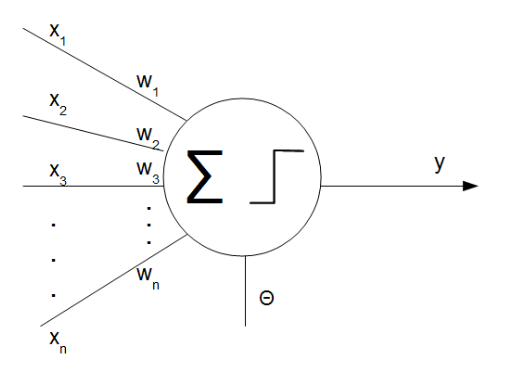
\includegraphics[height=6cm]{figures/perceptron.png}
\caption{McCulloch-Pittsův perceptron}
\label{fig:perceptron}
\end{center}
\end{figure}

Na vstupy neuronu se přivádí data ze vstupní množiny. Data mohou být i binární [0,1], nebo spojitá na intervalu <0,1>. Každý vstup \begin{math} x_{i}\end{math} je modifikován vahou daného vstupu \begin{math} w_{i}\end{math}. Tyto váhy vstupů se během učení mění, což představuje základ učení neuronu. Významným vstupům, které výrazně ovlivňují výstup neuronu se přiřazuje vyšší váha a naopak méně významným vstupům se váha snižuje.

Práh je hodnota, po jejímž překročení se neuron stává aktivním. Hodnota prahu se počítá jako vážený součet vstupů. Pokud tento součet nepřekročí prahovou hodnotu, zůstává neuron neaktivní. Práh je často realizován jako další vstup neuronu s konstantní hodnotou \begin{math} x_{0}=1\end{math}, váha \begin{math} w_{0}\end{math} potom označuje samotný práh. Funkce pro výpočet výstupu poté vypadá následovně:

\begin{equation}
  y=S(\sum\limits_{i=0}^N w_{i}x_{i}),\; kde\; x_{0}=1\mbox{.}
\end{equation}

Přenosová funkce je funkce, pomocí které je transformován vnitřní potenciál neuronu do požadovaného oboru hodnot. Pomocí vhodné volby přenosové funkce může neuron produkovat binární nebo spojitý výstup. Pro binární výstup se používají skoková a Heavisideova funkce, pro spojitý výstup se používají saturovaná lineární funkce, Gaussovská funkce, sigmoidní funkce a hyperbolický tangens.\citep{teoret}

\section{Proces učení}
Při učení dochází v neuronové síti ke změnám, kterými se síť adaptuje na řešení daného problému. Učení je u umělé neuronové sítě realizováno nastavováním vah a prahů jednotlivých neuronů. Během učení nedochází nikdy ke změně struktury sítě (s výjimkou sítě GMDH, která není v tomto textu rozebírána). Před začátkem učení se obvykle nastaví váhy a prahy neuronů na náhodné hodnoty.

U učení umělé neuronové sítě můžeme pozorovat paralelu s učením biologické neuronové sítě, kdy v obou případech dochází k opakovanému předkládání vstupních dat a kontrole výstupu. Tímto opakováním se obě sítě učí dokud nereagují na předávané vstupy správně, nebo jen s akceptovatelnou odchylkou, tedy dokud nejsou naučeny.

Existují dva způsoby učení neuronové sítě:
\begin{itemize}
\item Učení s učitelem

Při učení s učitelem máme k dispozici trénovací množinu, která se skládá ze vstupních vektorů a jim odpovídajících výstupních vektorů. Učení probíhá postupným předkládáním trénovacích vzorů. Ke každému vzoru ve vypočte odchylka od požadovaného výstupu a na základě této odchylky se upravují hodnoty vah. Váhy se upraví tak, aby při opětovném předložení vzoru byla odchylka od požadovaného výstupu menší. Tato úprava se řídí učicím algoritmem (probrán dále). Změna vah při jednom učicím kroku je obvykle malá. Poté se předloží nový vzor a celý proces se opakuje. Učicí vzory jsou síti předkládány opakovaně a po provedení dostatečného počtu opakování začne síť podávat stabilní výstup v reakci na předkládaný vstup.

\item Učení bez učitele

Při učení bez učitele nemá neuronová síť žádné vnější kritérium správnosti, má k dispozici pouze vstupní vektory. Síť tedy operuje pouze s informacemi, které získala během učení. Algoritmus učení bez učitele je navržen tak, aby hledal ve vstupních datech vzorky se společnými vlastnostmi. Učení bez učitele je také nazýváno samoorganizací.
\end{itemize}
Existuje také učení jednorázové, kdy je síti předložen vzor a síť si jej zapamatuje. Takováto schopnost učení je u neuronových sítí poměrně neobvyklá. Jednorázového učení je schopna například Hopfieldova síť.
\section{Proces vybavování}
Vybavování je aktivní fází neuronové sítě a zpracovávají se v ní vstupní data. Neuronová síť, stejně jako lidská mysl, pracuje asociativním způsobem.\citep{skripta} Asociativní paměť pracuje na principu asociovaných prvků např. obličej a jméno člověka, které si po spatření obličeje vybavíme.

Vybavování je možné rozlišit do dvou variant:
\begin{itemize}
\item Autoasociativní vybavování

Při autoasociativním vybavování dochází k vybavování stejného vektoru, který je předložen. Toto se může zdát nepraktické. Tuto vlastnost ale oceníme pokud je náš vzor poškozený nebo neúplný a neuronová síť nám ho dovede opravit. K tomuto účelu se také autoasociativní vybavování používá.
\item Heteroasociativní vybavování

Při heteroasociativním vybavování dochází po předložení vzoru k vybavení jiného vzoru, který je s předloženým asociován. Typickým použitím této varianty vybavování je klasifikace vektorů do tříd.
\end{itemize}

\section{Učicí algoritmy}
Nyní již víme, že neuronová síť se učí pomocí změn vah vstupů u jednotlivých neuronů. Abychom mohli pozorovat a měřit rozdíly v úspěšnosti sítě v průběhu učení, je potřeba zavést nějakou metriku, pomocí které budeme úspěšnost sítě měřit. V praxi se jako metrika používá střední kvadratická chyba (anglicky Mean Squared Error, odtud skratka MSE). MSE sítě se spočítá pomocí následující rovnice:
\begin{equation}
	MSE=\frac{1}{n}\sum\limits_{i=1}^n (y_{i}-o_{i})^{2}\mbox{,}
\end{equation}
 kde \begin{math}n\end{math} je počet vektorů v trénovací množině,  \begin{math}y_{i}\end{math} je výstup sítě po přivedení \textit{i}-tého prvku testovací množiny na vstup a \begin{math}o_{i}\end{math} je požadovaný výstup po přivedení \textit{i}-tého prvku z testovací množiny.

Výše uvedený vzorec je platný pro síť s jedním výstupním neuronem, pokud má síť výstupních neuronů více, sčítá se chyba na všech výstupních neuronech podle následujícího vzorce:
\begin{equation}
	MSE=\frac{1}{n}\sum\limits_{j=1}^m\sum\limits_{i=1}^n (y_{ji}-o_{ji})^{2}\mbox{,} 
\end{equation}
kde \begin{math}m\end{math} je počet neuronů výstupní vrstvy, n je počet vzorů v trénovací množině, \begin{math}y_{ji}\end{math} je výstup \textit{j}-tého neuronu po přivedení \textit{i}-tého prvku trénovací množiny a \begin{math}o_{ji}\end{math} je požadovaný výstup \textit{j}-tého neuronu po přivedení \textit{i}-tého prvku trénovací množiny.

Ještě výhodnější metrikou pro měření úspěšnosti sítě během trénování je RMSE (Root Mean Squared Error). Její největší předností je možnost přímo ji porovnat s výstupem sítě, protože je ve stejných jednotkách jako výstup. Hodnota RMSE se spočte následovně:
\begin{equation}
RMSE=\sqrt{MSE}\mbox{.}
\end{equation}
Platí, že čím nižší hodnota RMSE, tím lépe je neuronová síť naučena. Učicí algoritmy se v průběhu učení snaží minimalizovat hodnotu RMSE, rozdíl mezi jednotlivými algoritmy tedy spočívá v postupu, jakým je tato hodnota minimalizována. Všechny popisované algoritmy pracují iterativně.
\subsection{Algoritmus nejvyššího poklesu}
Algoritmus začíná s náhodně inicializovaným vektorem vah neuronů a vyžaduje zadat výchozí velikost učicího kroku. V každé iteraci je vektor vah neuronů upraven tak, aby se posunul ve směru nejvyššího poklesu funkce MSE o velikost učicího kroku, pokud by toto posunutí nesnížilo hodnotu MSE, je velikost učicího kroku snížena na polovinu. Snižování probíhá dokud posunutí váhového vektoru nezpůsobí pokles hodnoty funkce MSE.  Na závěr iterace je velikost učicího kroku zdvojnásobena, čímž je získána předběžná velikost kroku pro příští iteraci. Algoritmus končí pokud dosáhne minima funkce MSE (může být lokální minimum) nebo vyčerpá přidělený počet iterací.

Algoritmus nejvyššího poklesu je nejjednodušší algoritmus ze zde popisovaných. Potřebuje nejméně výpočetního výkonu a dosahuje mnohem horších výsledků než ostatní popisované algoritmy.\cite{nndocumentation}
\subsection{Gauss-Newtonův algoritmus}
Algoritmus začíná s náhodně inicializovaným vektorem vah. Na začátku každé iterace je nastavena velikost učicího kroku na hodnotu 1. Pro určení směru posunu je použita Gauss-Newtonova metoda(rozebrána v\citep{learningmachines}), která pro výpočet využívá první a druhé derivace. Ve vypočteném směru je vektor vah posunut o velikost učicího kroku. Posun je uskutečněn pouze pokud způsobí pokles hodnoty funkce MSE, jinak je velikost kroku snížena o polovinu. Poté algoritmus pokračuje další iterací. Algoritmus končí pokud dosáhne minima funkce MSE (může být lokální minimum) nebo vyčerpá přidělený počet iterací.

Gauss-Newtonův algoritmus je rychlý a spolehlivý algoritmus, který je využívaný v mnoha oblastech k řešení problémů s minimalizací funkcí. Pro řešení problémů v oblasti neuronových sítí nemusí být vždy nejvhodnější volbou, protože může docházet k výpočtům s hodnotami s velkým číselným rozsahem. Pokud k tomu dojde, bude algoritmus konvergovat velmi pomalu a bude zdržovat celý učicí proces.\cite{nndocumentation}
\subsection{Levenberg-Marquardtův algoritmus}
Algoritmus začíná, stejně jako předchozí algoritmy, s náhodně inicializovaným vektorem vah. Levenberg-Marquardtův algoritmus představuje kompromis mezi dvěma předchozími algoritmy. Výsledný směr posunutí vektoru vah je zjednodušeně dán kompromisem mezi směry, které navrhují algoritmus nejvyššího poklesu a Gauss-Newtonův algoritmus.  Namísto velikosti učicího kroku, která je u tohoto algoritmu stále 1, se mění hodnota \begin{math}\lambda\end{math}. Na začátku každé iterace se algoritmus pokusí snížit hodnotu \begin{math}\lambda\end{math}, pokud by takováto snížená hodnota \begin{math}\lambda\end{math} nezaručila pokles MSE, je \begin{math}\lambda\end{math} naopak zvětšována dokud nedojde k žádanému poklesu. Hodnota \begin{math}\lambda\end{math} určuje, kterému z navrhovaných směrů bude algoritmus přikládat vyšší váhu. Pokud se \begin{math}\lambda\end{math} blíží k nule, chová se algoritmus jako Gauss-Newtonův algoritmus, pokud \begin{math}\lambda\end{math} dosahuje vysokých hodnot, chová se jako algoritmus nejvyššího poklesu. Algoritmus končí za stejných podmínek jako Gauss-Newtonův algoritmus.\cite{nndocumentation}\cite{learningmachines} 

Levenberg-Marquardtův algoritmus představuje pravděpodobně nejlepší volbu trénovacího algoritmu pro neuronové sítě.

\subsection{Algoritmus zpětné propagace}
Algoritmus zpětné propagace začíná stejně jako ostatní algoritmy s náhodně inicializovaným vektorem vah. Před začátkem běhu je algoritmu třeba nastavit délku učicího kroku a momentum. Algoritmus zpětné propagace se chová velmi podobně jako algoritmus nejvyššího poklesu. Také sleduje směr nejvyššího poklesu funkce MSE, ale liší se v délce učicího kroku, která zůstává po celý běh algoritmu stejná. Momentum slouží jako jakási setrvačnost, která nám říká, jak dlouho se budeme držet určitého směru, než zabočíme ve směru nejvyššího poklesu. Díky momentu dokáže algoritmus opustit některá lokální minima. 

Algoritmus zpětné propagace je jedním z nejstarších algoritmů pro učení neuronových sítí. I přes použití momenta, které umožní uniknutí z lokálního minima, se nedoporučuje algoritmus zpětné propagace používat. Namísto zpětné propagace se doporučuje použít některý z moderních učicích algoritmů a opakovat trénink pro několik různých, náhodně inicializovaných vektorů vah.\cite{nndocumentation} Podrobnější popis algoritmu naleznete v\citep{skripta}.
%*****************************************************************************
\chapter{Neuronové sítě}
\section{Dopředná síť}
Dopředná neuronová síť se zpětným šířením chyby, někdy také nazývána síť Back-propagation podle pravděpodobně nejznámějšího algoritmu, který je k učení této sítě využíván, patří mezi vícevrstvé neuronové sítě. Dopředná síť má alespoň jednu skrytou vrstvu neuronů. Dopředná neuronová síť, jak již název napovídá, využívá dopředného šíření signálu. Tato neuronová síť je velmi flexibilní v možnostech použití a je poměrně jednoduchá. Díky těmto vlastnostem je jednou z nejpoužívanějších sítí v praxi.

\subsection{Topologie sítě}
Síť je složena z McCulloch-Pittsových neuronů, které využívají jako aktivační funkci sigmoidu. Neurony v dopředné síti jsou tedy spojité. Dopředná neuronová síť se skládá minimálně ze tří vrstev - vstupní, skryté a výstupní. Strukturu sítě skládající se ze čtyř vrstev můžete vidět na obrázku~\ref{fig:ffschema}. Sousední vrstvy jsou mezi sebou propojeny - každý neuron z vyšší vrstvy je propojen s každým neuronem v nižší vrstvě. První vrstva tzv. vstupní vrstva slouží pouze k rozdělení vstupního signálu a jeho přivedení na neurony první skryté vrstvy. Neurony v ostatních vrstvách sítě jsou již výkonné prvky, na kterých probíhá učení.
\begin{figure}[!h]
\begin{center}
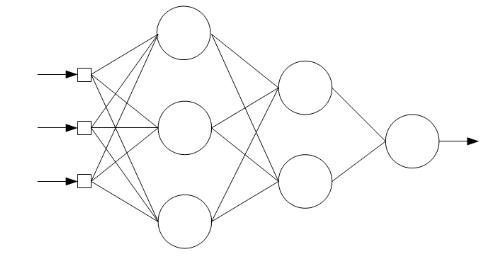
\includegraphics[height=4.5cm]{figures/ffschema.png}
\caption{Schéma dopředné neuronové sítě}
\label{fig:ffschema}
\end{center}
\end{figure}

Počet použitých skrytých vrstev se liší případ od případu. Zvolení vhodného počtu vrstev je většinou provedeno experimentálně. Pro počet neuronů ve skrytých vrstvách existují doporučení. Následující doporučení je pro síť s jednou skrytou vrstvou:
\begin{equation}
N_{skryt}=\sqrt{N_{vst}\cdot N_{vyst}} \mbox{,}
\end{equation}
kde \begin{math}N_{skryt}\end{math} je doporučený doporučený počet ve skryté vrstvě, \begin{math}N_{vst}\end{math} je počet neuronů ve vstupní vrstvě a \begin{math}N_{vyst}\end{math} je počet neuronů ve výstupní vrstvě. Pro síť s dvěma skrytými vrstvami se doporučují následující počty neuronů.
\begin{equation}
N_{skryt-1}=N_{vyst}\cdot\left(\sqrt[3]{\frac{N_{vst}}{N_{vyst}}}\right)^{2} \,\mbox{a} \,\,\,\,\,\, N_{skryt-2}=N_{vyst}\cdot\left(\sqrt[3]{\frac{N_{vst}}{N_{vyst}}}\right)\mbox{.}
\end{equation}
Tato doporučení představují většinou horní odhady a lépe je určit počty neuronů experimentálně.\citep{skripta}

Dopředné šíření signálu probíhá následovně. Nejprve je vstupní vektor přiveden na vstupní vrstvu, tato vrstva vstup přenese na první skrytou vrstvu. Na skryté vrstvě dojde k úpravě tohoto signálu podle váhových vektorů jednotlivých neuronů, výstup těchto neuronů je přenesen na další vrstvu. Takto se dostanou data postupně až na výstup poslední (výstupní) vrstvy, odkud je výstup odebrán.

Učení sítě probíhá s učitelem a využívá se k němu jeden z algoritmů popsaných v předchozí kapitole.
\section{RBF síť}
RBF (Radial Basis Function) neuronové sítě jsou známe od 80. let dvacátého století. Jejich rozvoj je spjat s výzkumem tzv. radiálních basických funkcí, které jsou použity jako aktivační funkce neuronů. Síť využívá dopředného šíření signálu a její učení probíhá s učitelem. RBF neuronové sítě představují přímou konkurenci pro dopředné neuronové sítě, protože jsou využívány na stejné úlohy (hlavně klasifikace a aproximace) a jejich učení je výrazně rychlejší než u dopředných sítí.

\subsection{Topologie sítě}
RBF síť se skládá vždy ze tří vrstev neuronů a využívá dopředné šíření signálu. První vrstva je vstupní a slouží pouze k  rozvedení signálu do druhé vrstvy. Druhá vrstva je skrytá a obsahuje RBF neurony (popsány níže). Vstupní a skrytá vrstva jsou úplně propojeny, každý vstupní neuron je propojen s každým RBF neuronem. Výstup z RBF neuronů je přiveden na neurony výstupní vrstvy (popsány níže), které z nich vypočtou výstup sítě. RBF vrstva je obvykle úplně spojena s výstupní vrstvou, ale v případě potřeby je možné některý ze spojů vynechat. Topologii sítě přibližuje obrázek~\ref{fig:rbfschema}.
\begin{figure}[!h]
\begin{center}
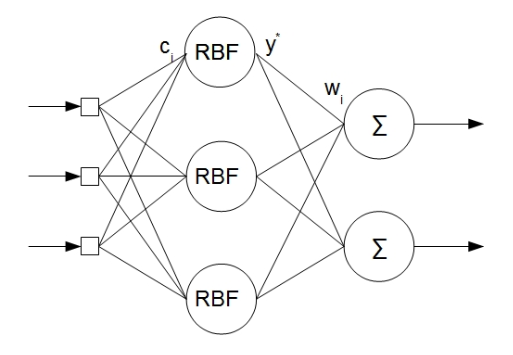
\includegraphics[height=4.5cm]{figures/rbfschema.png}
\caption{Schéma RBF neuronové sítě}
\label{fig:rbfschema}
\end{center}
\end{figure}
\subsubsection{RBF neuron}
RBF neuron se od McCulloch-Pittsova neuronu nejvíce odlišuje v použité aktivační funkci a způsobu výpočtu vnitřního potenciálu neuronu. Vnitřní potenciál neuronu se vypočte následovně:
\begin{equation}
\varphi =\sqrt{\sum\limits_{i=1}^n(x_{i}-c_{i})^{2}} \mbox{,}
\end{equation}
kde \begin{math}\varphi\end{math} je vnitřní potenciál neuronu, \begin{math}x_{i}\end{math} je \textit{i}-tý prvek vstupního vektoru a 
\begin{math}c_{i}\end{math} je váha \textit{i}-tého vstupu RBF neuronu. Vidíme, že vnitřní potenciál udává Eukleidovská vzdálenost předloženého vektoru od vektoru vah RBF neuronu (tento vektor se někdy také nazývá prototyp, protože je reprezentantem určité podmnožiny dat ve formě shluku).

Jako aktivační funkce se nejčastěji používá Gaussova funkce, která je známa ze statistiky. Gaussova funkce má následující rovnici:
\begin{equation}
y^{*}=e^{-\frac{\varphi^{2}}{\sigma^{2}}}\mbox{,}
\end{equation}
kde \begin{math}y^{*}\end{math} určuje výstup RBF neuronu, \begin{math}\varphi\end{math} je hodnota vnitřního potenciálu neuronu a \begin{math}\sigma\end{math} je parametr, který určuje strmost Gaussovy funkce. Gaussova funkce je výhodná, protože určuje míru příslušnosti vzoru k prototypu. Pokud je vzor totožný s prototypem, nabývá hodnota Gaussovy funkce hodnoty 1, se vzrůstající vzdáleností vzoru od prototypu hodnota funkce klesá. Kromě Gaussovy funkce se jako aktivační funkce používají ještě další funkce. Jednou z nich je funkce:
\begin{equation}
y^{*}=\varphi
\end{equation}, kdy se aktivita neuronu se vzrůstající vzdáleností vzoru od prototypu zvyšuje.

\subsubsection{Neuron výstupní vrstvy}
Neurony ve výstupní vrstvě jsou perceptronovského typu a jejich výstup je definován rovnicí:
\begin{equation}
y=\sum\limits_{i=1}^n(w_{i}y^{*}_{i})\mbox{,}
\end{equation}
kde \begin{math}w_{i}\end{math} je váha daného vstupu, \begin{math}y^{*}_{i}\end{math} je výstup RBF neuronů a \textit{y} je výstup neuronové sítě.
\subsection{Učení RBF sítě}
Učení RBF sítě se provádí s učitelem. K učení sítě je potřeba stejná množina trénovacích dat, jaká je používána pro učení dopředné sítě. Učení RBF sítě se dělí do dvou fází.\cite{skripta} V první fázi se nastavují váhové vektory \begin{math}c_{i}\end{math} u RBF neuronů, ve druhé fázi se učí neurony výstupní vrstvy.
\begin{itemize}
\item 1. fáze

V této fázi je potřeba určit pozice prototypů. K tomuto účelu se využívá adaptivní K-means algoritmus, používaný především ke shlukové analýze. Tento algoritmus zde bude popsán jen obecně, podrobný popis algoritmu, včetně rovnic, naleznete v\cite{skripta}. Algoritmus K-means se skládá z následujících čtyř kroků:
\begin{enumerate}
\item Náhodně se inicializují pozice prototypů.
\item Načte se jeden vzor z trénovací množiny.
\item Určí se prototyp, který je načtenému vzoru nejblíže. Tento prototyp se posune o \begin{math}\eta\end{math} násobek vzdálenosti vzor-prototyp směrem ke vzoru.
\item Konec pokud \begin{math}\eta =0\end{math}, nebo po určitém počtu iterací. Jinak se pokračuje bodem 2.
\end{enumerate}
Velikost \begin{math}\eta\end{math} se v průběhu učení snižuje.

Velikost parametru \begin{math}\sigma\end{math} (strmost Gaussovy funkce) se vypočte pro každý shluk (neuron) jako střední kvadratická vzdálenost všech vektorů, patřících do shluku, od prototypu:
\begin{equation}
\sigma =\sqrt{\frac{1}{Q}\sum\limits_{q=1}^Q||\overline{C}-\overline{X}_{q}||^{2}} \mbox{,}
\end{equation}
kde \begin{math}C\end{math} je ptorotyp daného shluku, \begin{math}Q\end{math} udává počet prvků patřící do shluku a \begin{math}\overline{X}_{q}\end{math} je \textit{q}/tý vektor shluku.
Tato fáze učení probíhá formou samoorganizace tedy učením bez učitele.   
\item 2. fáze 

V této fázi dochází k učení pouze neuronů ve výstupní vrstvě, parametry RBF neuronů zůstávají po 1. fázi nezměněny. V této fázi probíhá učení s učitelem. K učení výstupní vrstvy je použit algoritmus nejvyššího sestupu popsaný v předchozí kapitole.
\end{itemize} 

\section{Hopfieldova síť}
Hopfieldova síť je pojmenována po svém objeviteli Johnu Hopfieldovi. Síť funguje jako autoasociativní paměť a používá se převážné ke zpracovávání obrazových vstupů. Díky svým vlastnostem je síť používána k čištění zašuměných vzorů nebo k rekonstrukci neúplných vzorů. Také je možné použít ji k řešení optimalizačních problémů.

\subsection{Topologie sítě}
Hopfieldova síť se skládá z McCulloch-Pittsových perceptronů, má stejně neuronů jako má vstupů, pokud tedy učíme síť obrázky 8\begin{math}\times\end{math}8 pixelů, má síť 64 neuronů. Každý neuron je pouze jedním svým vstupem napojen na vstup sítě. Výstup z každého neuronu je veden přes synaptické váhy \begin{math}w_{ij}\end{math} na vstup všech ostatních neuronů, čímž se vytváří zpětnovazební smyčky. Síť má tedy symetrickou strukturu. Protože je Hopfieldova síť autoasociativní, musí mít stejně vstupů jako výstupů, každý neuron v síti má tedy kromě jednoho vstupu také jeden výstup. Hodnoty prahů neuronů jsou nulové, přenosovou funkcí je nejčastěji dvouhodnotová skoková funkce. Strukturu sítě znázorňuje obrázek~\ref{fig:hopfieldstr}.

\begin{figure}[!h]
\begin{center}
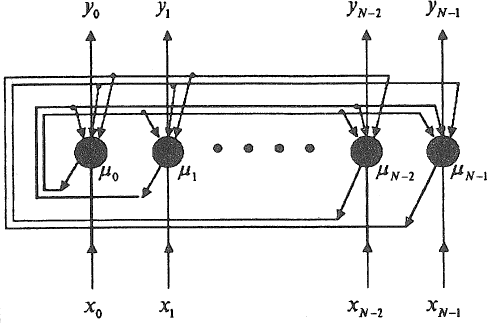
\includegraphics[height=6.5cm]{figures/hopfield.png}
\caption{Struktura Hopfieldovy neuronové sítě\cite{skripta}}
\label{fig:hopfieldstr}
\end{center}
\end{figure}
\begin{math}x_{0},x_{1},...,x_{n-1}\end{math} jsou vstupy sítě, \begin{math}\mu _{0},\mu _{1},...,\mu _{n-1}\end{math} jsou stavy v jednotlivých krocích, které se v následujícím kroku stanou vstupy. Výstupy \begin{math}y_{0},y_{1},...,y_{n-1}\end{math} jsou neaktivní, dokud nedojde k vybavení vzoru. Vybavování je u Hopfieldovy neuronové sítě iterativní proces. Jakmile skončí proces vybavování, jsou výstupy \begin{math}y_{0},y_{1},...,y_{n-1}\end{math} nataveny na hodnoty \begin{math}\mu _{0},\mu _{1},...,\mu _{n-1}\end{math}.

\subsection{Učení Hopfieldovy sítě}
Hopfieldova neuronová síť si uchovává informace v podobě matice vah mezi jednotlivými neurony. Matice má dimenzi N\begin{math}\times\end{math}N, kde N je počet neuronů v síti. Tato matice má na diagonále nuly (žádný neuron není spojen sám se sebou) a je diagonálně souměrná protože dva neurony mají mezi sebou vždy nastavenu stejnou váhu (platí že \begin{math}w_{ij}=w_{ji}\end{math})

Způsob učení a vybavování si ukážeme na jednodušším binárním modelu.

Učení každého vzoru v Hopfieldově síti probíhá jednorázově. Vzor je předložen a síť se ho naučí. Neuronová síť se učí pomocí změny matice vah. Matice vah naučené sítě získáme součtem dílčích matic vah. Pro každý učený vzor získáme dílčí matici vah následujícím způsobem:
\begin{equation}
w_{ij} = \left\{ 
\begin{array}{l l}
  x_{i}x_{j} &  \mbox{, pro $i\neq j$, }\\
  0 & \mbox{,  pro $i=j$, $i\leq0$, $j\leq N-1$}\\ \end{array} \right. \mbox{,}
\end{equation}
kde $w_{ij}$ je prvek dílčí váhové matice na pozici $i,j$ a $x_{i}$ resp. $x_{j}$ je \textit{i}-tý resp. \textit{j}-tý prvek na vstupu.

Tímto způsobem jsou předloženy všechny trénovací vzory, kterých je M. Pro získání výsledné matice nám stačí tyto dílčí matice sečíst, čímž získáme výslednou matici vah naučené sítě.

Při učení sítě si můžeme klást otázku kolik vzorů je síť schopna se naučit. Kapacita sítě samozřejmě není neomezená a závisí na počtu použitých neuronů. Experimentálně bylo zjištěno, že počet vzorů musí být nižší než 15\% počtu použitých neuronů\cite{skripta}, musí tedy platit vzorec:
\begin{equation}
P\approx 0.15N \mbox{,}
\end{equation}
kde \textit{P} je počet učených vzorů a \textit{N} je počet neuronů. Pokud by nebyl tento poměr dodržen, může se stát, že si síť bude vybavovat nesmyslné, nenaučené vzory.

Pokud budeme chtít naučit Hopfieldovu síť rozpoznávat všechny znaky české abecedy, kterých je 42 (včetně háčků a čárek), budeme podle předchozího vzorce potřebovat neuronovou síť o minimálně 280 neuronech. Z toho vyplývá, že matice vah bude mít \begin{math}280^{2}=78400\end{math} hodnot. Tím se dostáváme k největší nevýhodě Hopfieldovy sítě, kterou je nízká kapacita při vysokých paměťových nárocích. Další nevýhodou je nulová odolnost proti natočení nebo posunutí vstupu. Díky těmto vlastnostem se základní Hopfieldova síť téměř nepoužívá.
\subsection{Vybavování vzoru}
Vybavování vzoru u Hopfieldovy sítě je založeno na porovnávání vzorů pomocí Hammingovy vzdálenosti. Za správnou odpověď se považuje ten naučený vzor, který má Hammingovu vzdálenost od předloženého vzoru nejnižší.
Vybavování v Hopfieldově síti je iterační proces. Po předložení vzoru je tedy nutné počkat, dokud síť nedospěje ke svému výstupu.
Vybavování probíhá podle následujícího algoritmu\cite{skripta}:
\begin{enumerate}
\item Nastavení počátečních stavů neuronů podle předloženého vzoru:
\begin{equation}
\mu_{i}(0)=x_{i}\mbox{,}0\leq i\leq N-1 \mbox{,}
\end{equation}
kde $\mu_{i}(t)$ je stav \textit{i}-tého neuronu v čase \textit{t} a $x_{i}$ je element vzoru nabývající hodnoty $\pm 1$.
\item Iterování 
\begin{equation}
\mu_{i}(t+1)=f\left[\sum\limits_{j=0}^{N-1}w_{ij}\mu_{i}(t) \right]\mbox{, }0\leq i\leq N-1 \mbox{,}
\end{equation}
kde $f$ je skoková aktivační funkce. Tento krok provádíme dokud dochází ke změnám stavů. Jakmile nedojde při iteraci k žádné změně, je algoritmus vybavování ukončen.
\item Na výstupy sítě jsou předány vnitřní stavy jednotlivých neuronů.
\begin{equation}
y_{i}=\mu_{i}(t_{posledni})
\end{equation}
Nyní můžeme předložit další vzor k vybavování.
\end{enumerate}
\section{Samoorganizující mapa}
Samoorganizující mapa, zkráceně SOM (Self Organizing Map), byla objevena na počátku osmdesátých let dvacátého století. Jejím objevitelem je finský profesor Teuvo Kohonen, podle něho je také někdy nazývána Kohonenova síť nebo Kohonenova mapa. Samoorganizující mapa pracuje na principu shlukové analýzy. SOM se učí metodou bez učitele a využívá soutěžní strategii učení. V jeden časový okamžik je v síti pouze jeden neuron aktivní a neurony mezi sebou soutěží o to, který bude aktivní. Kohonen také formuloval algoritmus učení samoorganizující mapy, který si klade za cíl vytvoření množiny reprezentantů, kteří mají stejnou pravděpodobnost výběru.\cite{teoret} 

Samoorganizující mapy jsou nejčastěji používány k vizualizováni topologie a hierarchické struktury vícerozměrných dat. Vstupní data jsou pomocí samoorganizující mapy transformována do prostoru s nižší dimenzí (nejčastěji dvoudimenzionálního). Další možností využití je rozpoznávání řeči.\cite{skripta} 
\subsection{Topologie sítě}
Samoorganizující mapa se skládá ze dvou vrstev. První vrstvou je vrstva vstupní, ta pouze distribuuje vstupní vektor na vstupy každého neuronu ve druhé vrstvě. Tyto dvě vrstvy jsou tedy úplně propojeny. Druhá vrstva je někdy nazývána Kohonenova vrstva. Neurony v Kohonenově vrstvě jsou uspořádány (nejčastěji do dvoudimenzionální mřížky). Neurony mají tedy pevně definované sousedy. Každý neuron v Kohonenově vrstvě reprezentuje určitý bod (včetně jistého okolí) ve vstupním prostoru. Neuron v Kohonenově vrstvě má stejný počet vstupů jako samotná SOM. Váhy vstupů u neuronu slouží k uložení pozice bodu, který neuron reprezentuje. Přenosovou funkcí neuronu je Eukleidovská vzdálenost. Výstupem neuronu je Eukleidovská vzdálenost vektoru uloženého ve vahách vstupů a předkládaného vektoru. Výstupem celé sítě  je (podle principu vítěz bere vše) ten neuron, který má spočtenou Eukleidovskou vzdálenost nejmenší.
Strukturu Kohonenovy sítě ukazuje obrázek~\ref{fig:kohonen1}

\begin{figure}[!h]
\begin{center}
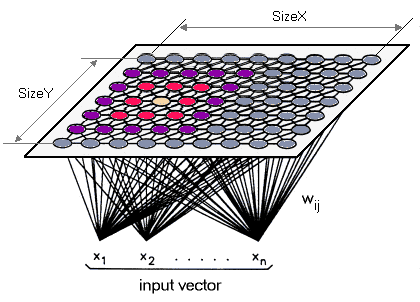
\includegraphics[height=5cm]{figures/kohonen1.png}
\caption{Struktura samoorganizující mapy\cite{SDL}}
\label{fig:kohonen1}
\end{center}
\end{figure}
\subsection{Učení sítě}
Učicí algoritmus se pokouší uspořádat neurony v mřížce do takové podoby, aby mřížka co nejlépe vystihovala vstupní data. Učení probíhá bez učitele a iterativně. Učicí algoritmus samoorganizující mapy je velmi jednoduchý, proto jej zde uvedeme pouze neformálně. Podrobnější popis algoritmu včetně rovnic naleznete v \cite{skripta}.

Nejprve se nastaví váhy vstupů u všech neuronů na náhodné hodnoty. Zvolí se velikost učicího kroku (tímto parametrem je možné ovlivnit rychlost učení sítě) a nastaví se velikost okolí neuronu tak, aby do tohoto okolí spadaly všechny ostatní neurony. Okolí neuronu si představme jako skupinu neuronů, které se nachází do určité vzdálenosti od zvoleného neuronu (příkladem okolí mohou být červené neurony na obrázku~\ref{fig:kohonen1}). Poté je neuronové síti předložen trénovací vzor. Vypočteme Eukleidovskou vzdálenost všech neuronů od předloženého vzoru a vybereme nejbližší neuron. Tomuto neuronu a všem neuronům v jeho okolí přizpůsobíme váhy směrem k předloženému vzoru o rozdíl odpovídajících si prvků vynásobený velikostí učicího kroku. Zmenšíme okolí a pokračujeme předložením dalšího vzoru.

Proces učení si můžeme představit jako rozprostírání původně zmačkaného papíru do roviny tak, aby pokrýval celý vstupní prostor.
\subsection{Vybavování vzorů}
Vybavování v samoorganizující mapě je velmi snadné, probíhá formou hledání reprezentanta pro předložený vektor. Tímto reprezentantem se stane neuron, jehož váhový vektor nejvíce odpovídá předloženému vzoru. Algoritmus vybavování je následující: Předloží se vstupní vektor, pro všechny neurony se vypočte Eukleidovská vzdálenost od vstupního vektoru a neuron s nejmenší Eukleidovskou vzdáleností vítězí a je vybrán jako reprezentant.
\section{Learning Vector Quantization (LVQ)}
Learning Vector Quantization (LVQ) je rozšířením samoorganizující mapy o učení s učitelem. Toto rozšíření navrhl stejně jako samoorganizující mapu Teuvo Kohonen. LVQ má k dispozici k učicím vzorům také jejich správné třídy, bude tedy moci klasifikovat i neznámá data. Struktura LVQ sítě je stejná jako struktura SOM.

Hlavní použití LVQ spočívá v klasifikaci dat.
\subsection{Učení sítě}
V prvním kroku učení se použije standardní algoritmus pro učení samoorganizující mapy. Pomocí tohoto algoritmu dojde k rozmístění reprezentantů (neuronů) v prostoru vstupních dat. V druhém kroku se znovu předloží vstupní data tentokrát i s informací o jejich příslušnosti ke třídě. Pro každý vstupní vektor se určí vítězný (nejbližší) neuron a zapamatuje se informace o příslušnosti vstupního vektoru ke třídě. Po tomto průchodu je pro každý neuron vytvořena tabulka četností tříd, které k tomuto neuronu náleží. Neuronu je přiřazena ta třída, kterou má v tabulce zastoupenu nejčastěji. Posledním krokem učení je zpřesnění pozic neuronů. K tomuto zpřesnění se používají tři algoritmy LVQ1, LVQ2 a LVQ3.
\begin{itemize}
\item LVQ1

U metody LVQ1 dojde k opětovnému předložení vzorů, pro každý vzor je vybrán neuron resp. jeho váhový vektor, který je předloženému vzoru podle Eukleidovské metriky nejblíže. Pouze tomuto vybranému neuronu upravíme váhový vektor podle následující rovnice:
\begin{equation}
w_{i}(t+1)=w_{i}(t)+\eta (t)\left[x_{i}(t)-w_{i}(t)\right]\mbox{,}
\end{equation}
pokud je vzor klasifikován dobře(učení),
\begin{equation}
w_{i}(t+1)=w_{i}(t)-\eta (t)\left[x_{i}(t)-w_{i}(t)\right]\mbox{,}
\end{equation}
pokud je vzor klasifikován spatně(odučení), kde $0<i<N-1$, $w_{i}$ jsou složky váhového vektoru neuronu, $x_{i}$ jsou složky vstupního vektoru a $\eta$ je parametr učení. Nejbližší neuron je tedy \uv{přisunut} k předloženému vzoru nebo je od něj \uv{odsunut}. Ostatním neuronům zůstávají jejich původní váhy.

Hranice vytvořená pomocí této metody se nachází ve středu spojnice dvou neuronů patřících do rozdílných tříd.
\item LVQ2

Metoda LVQ2 zpřesňuje metodu LVQ1. Na rozdíl od předchozí metody si metoda LVQ2 vybírá dva nejbližší neurony a úpravu vah provádí pouze v případě, kdy jeden neuron klasifikuje správně a druhý špatně. Předpokládejme dva váhové vektory $w^{1}_{i}$ a $w^{2}_{i}$ reprezentující dvě různé třídy $T_{1}$ a $T_{2}$. Rozhodovací hranice mezi nimi je zde nahrazena okénkem (pásem), které má nenulovou šířku (šířka se určuje experimentálně\cite{skripta}) a jehož středem prochází hranice. Algoritmus uvažuje modifikaci vektorů pouze pokud vstupní vektor leží v okénku a patří do opačné třídy než vektor, který je mu nejblíže. Váhy neuronů jsou poté upraveny následovně:
\begin{equation}
w_{i}^{1}(t+1)=w_{i}^{1}(t)-\eta (t)\left[x_{i}(t)-w_{i}^{1}(t)\right]\mbox{,}
\end{equation}
odsunutí chybně klasifikujícího neuronu od vstupního vektoru,
\begin{equation}
w_{i}^{2}(t+1)=w_{i}^{2}(t)+\eta (t)\left[x_{i}(t)-w_{i}^{2}(t)\right]\mbox{,}
\end{equation}
přisunutí správně klasifikujícího neuronu k vstupnímu vektoru, kde $x_{i}$ jsou složky vstupního vektoru, $0<i<N-1$ a $\eta$ je velikost učicího kroku. Ostatní neurony zůstávají beze změny.

Algoritmus zprvu skutečně zlepšuje pozici hranice mezi třídami. Po větším počtu iterací se však začne pozice hranice zhoršovat. Proto je výhodné použít tento algoritmus jen pro menší počat iterací (např. 10000)\cite{courseware}.
\item LVQ3

Z důvodu nestability metody LVQ2 pro pro velký počet iterací vznikl algoritmus LVQ3, který tento nedostatek odstraňuje. Algoritmus LVQ3 rozšiřuje algoritmus LVQ2 o pravidlo, které zajišťuje přibližování správně klasifikujících neuronů k tréningovým vzorům.Rozšiřující pravidlo je následující:

V případě, kdy předložený vzor i oba nejbližší neurony mají stejnou třídu, proveď u obou neuronů následující úpravy:
\begin{equation}
w_{i}(t+1)=w_{i}(t)+\lambda \eta(t)\left[x_{i}(t)-w_{i}(t)\right]\mbox{,}
\end{equation}
kde hodnota koeficientu $\lambda\in\left\lbrace0.1,0.5\right\rbrace$ je přímo úměrná velikosti okénka, její hodnota byla odhadnuta experimentálně.\cite{skripta}

Algoritmus LVQ3 je již dostatečně stabilní, tzn. že po nalezení optimálního váhového vektoru neuronu se již tato hodnota nebude měnit.
\end{itemize}
%*****************************************************************************
\chapter{Učení a hodnocení sítě}
\section{Rozdělení vstupních dat}
Po naučení neuronové sítě je vhodné vědět jak dobře bude síť vykonávat činnost, kterou byla naučena. K tomuto vyhodnocení bychom ideálně potřebovali další vstupní data (pro síť neznámá), pomocí kterých bychom změřili úspěšnost sítě. Tato data většinou k dispozici nemáme, proto je potřeba si je nějak obstarat. Tato testovací data se získají rozdělením množiny dat, kterou máme k dispozici k učení sítě, na dvě menší množiny tzv. trénovací a testovací množinu. V jakém poměru data rozdělit je závislé na mnoha faktorech, v praxi se často tento poměr určuje experimentálně. Učení sítě je poté provedeno na trénovací množině a na testovací množině je určena skutečná chybovost sítě.

Jedním z nebezpečí při učení neuronové sítě je její přeučení. Přeučení sítě znamená, že je síť příliš přizpůsobena trénovacím datům (např. se přizpůsobila šumu v datech). Takto přeučená síť poté podává výborné výsledky na trénovacích datech, v praxi nebo na testovacích datech by již byly její výsledky podstatně horší. Tomuto problému je možné předejít použitím validační množiny. Validační množina slouží k ověření úspěšnosti sítě během učení. V každé iteraci učicího algoritmu je vyhodnocena úspěšnost sítě na validační množině a v případě, že by provedením iterace došlo ke zvýšení chyby na validačních datech, není již tato iterace provedena a síť je prohlášena za naučenou. Druhou možností je nechat proběhnout požadovaný počet iterací učicího algoritmu, v jeho průběhu sledovat vývoj chyby na validační množině a za naučenou síť prohlásit síť v té iteraci, kdy byla chyba na validačních datech nejmenší.
Jako validační množinu je možné použít testovací množinu. Pokud chceme striktně dodržet postup, že neuronová síť nesmí v průběhu učení přijít do styku s testovací množinou, je možné validační množinu získat jako podmnožinu trénovacích dat.
\section{Křížová validace}
Při učení sítě může mít významnou roli na její úspěšnost náhodné rozdělení dat na trénovací, testovací a případně validační množinu nebo náhodná počáteční inicializace sítě.
Křížová validace může sloužit právě k omezení vlivu těchto náhodných jevů na odhad úspěšnosti sítě, nejčastěji je však využívána k nastavení parametrů různých algoritmů. V našem případě ji tedy můžeme použít k vybrání nejlepší struktury sítě. Křížová validace probíhá následujícím způsobem:
\begin{enumerate}
\item Trénovací data se náhodně rozdělí do $k$ stejně velkých množin. Hodnota $k$ určuje stupeň křížové validace. Množiny dat se nazývají foldy.
\item Pro každý fold je vytvořena náhodně inicializovaná neuronová síť, která je na zbývajících foldech naučena a tento jeden fold slouží jako testovací množina, pro určení úspěšnosti sítě.
\item Z úspěšností sítě pro všechny foldy se spočte průměr. Tento průměr je neovlivněným odhadem úspěšnosti dané sítě.
\end{enumerate}
Existuje několik různých typů křížové validace:
\begin{itemize}
\item K-stupňová křížová validace je popsána výše.
\item Stratifikovaná křížová validace. Při stratifikované křížové validaci jsou data rozdělena do foldů tak, aby v každém foldu byly třídy zastoupeny ve stejném poměru jako v trénovacích datech.
\item Leave-one-out křížová validace je extrémní případ k-stupňové křížové validace, kde k je rovno počtu vektorů v trénovacích datech.
\end{itemize}
%*****************************************************************************
\chapter{Implementační prostředí}
\section{Wolfram Mathematica}
Systém Mathematica od firmy Wolfram Research je sofistikovaný matematický nástroj, který umožňuje provádět numerické i symbolické výpočty. Systém obsahuje velké množství vestavěných funkcí a umožňuje i přidání dalších uživatelsky definovaných funkcí. Dále nabízí široké možnosti vizualizace dat ve 2D i 3D grafech. Prostředí systému vidíte na obrázku~\ref{fig:prostredi}. Neméně podstatnou funkcí je možnost exportu vyhodnoceného notebooku do formátu pdf. Díky tomu může demonstrační aplikaci vytvořenou v systému Mathematica, byť v omezené míře, využít i student, který nemá na svém počítači systém Mathematica nainstalovaný. Systém je možné rozšířit celou řadou knihoven, jednou z nich je i knihovna Neural Networks, kterou jsem využil ve své demonstrační aplikaci. Demonstrační aplikaci jsem programoval ve verzi Mathematica 8.0. Pro studium programování v Mathematice jsem použil knihy\cite{mathD} a \cite{mathP}.

\begin{figure}[!h]
\begin{center}
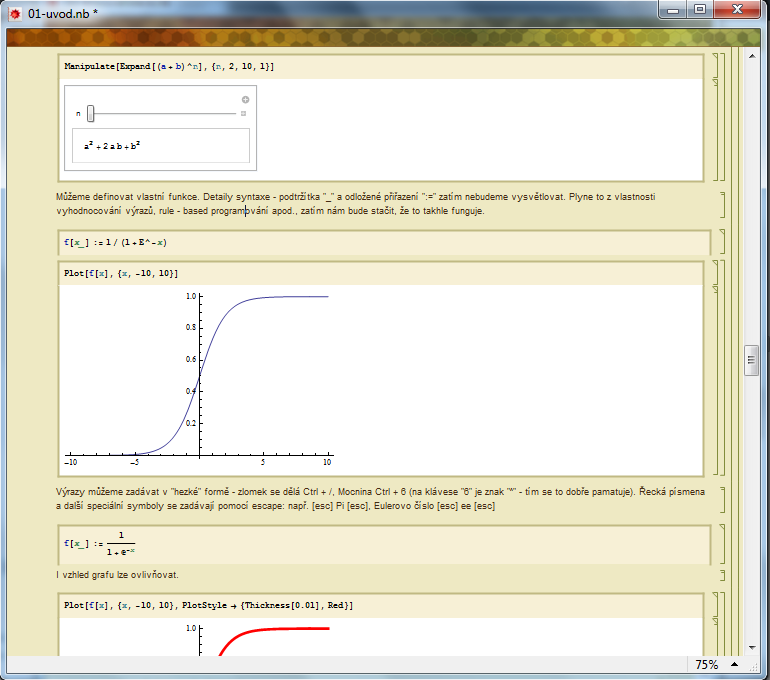
\includegraphics[height=10cm]{figures/ukazka01.png}
\caption{Ukázka prostředí systému Mathematica}
\label{fig:prostredi}
\end{center}
\end{figure}

\section{Knihovna Neural Networks}
Knihovna Neural Networks rozšiřuje systém \textit{Mathematica} o možnost pracovat s neuronovými sítěmi bez nutnosti vytvářet si její vlastní implementaci. Konkrétně knihovna nabízí práci s těmito konkrétními sítěmi: jednoduchý perceptron, dopředná neuronová síť, RBF neuronová síť, Hopfieldova neuronová síť, dynamická neuronová síť, Kohonenova mapa, LVQ a VQ. Knihovna také poskytuje implementaci různých algoritmů učení sítě, konkrétně jsou to tyto algoritmy: Levenberg-Marquardtův, Gauss-Newtonův, algoritmus nejvyššího poklesu a algoritmus zpětné propagace. Knihovna umožňuje široké možnosti natavení parametrů u jednotlivých sítí a pro méně zkušené uživatele nabízí vytvoření sítě s výchozími parametry. Výchozí parametry jsou voleny tak, aby síť s výchozími parametry podávala dobré výkony a její učení a vybavování netrvalo přehnaně dlouho. Knihovna ještě nabízí široké možnosti vizualizace dat, grafické zobrazení průběhu učení sítě a také grafické zobrazení výstupu naučené neuronové sítě. Ke knihovně patří návod k použití a rozsáhlá dokumentace.
%*****************************************************************************
\chapter{Experimenty s neuronovými sítěmi}

\begin{center}
\begin{table}[h]
\begin{tabular}{|c|l|l|}
\hline 
Číslo kapitoly & Název kapitoly & Soubor \\ \hline
1 & Úvod & 01-uvod.nb \\ \hline
2 & Algoritmy učení & 02-algoritmy-uceni.nb \\ \hline
3 & Křížová validace & 03-krossvalidace.nb \\ \hline
4 & Dopředná síť a umělá data sin(x) & 04-feedforward-sin.nb \\ \hline
5 & Dopředná síť a Iris data & 05-feedforward-iris.nb \\ \hline
6 & Přístupy k učení dopředné sítě & 06-feedforward-iris-2.nb \\ \hline
7 & Pokrytí dat jednoduchou RBF sítí & 07-rbf-neuron.nb \\ \hline
8 & Pokrytí dat RBF sítí & 08-rbf-neuron-2.nb \\ \hline
9 & Síť RBF a umělá data sin(x) & 09-rbf-sin.nb \\ \hline
10 & Síť RBF  Iris data & 10-rbf-iris.nb \\ \hline
11 & Přístupy k učení RBF sítě & 11-rbf-iris-2.nb \\ \hline
12 & Hopfieldova síť a umělé vzory & 12-hopfield.nb \\ \hline
13 & Shlukování dat sítí bez učitele & 13-som-clustering.nb \\ \hline
14 & Kohonenova síť a Iris data & 14-som-iris.nb \\ \hline
15 & LVQ a Iris data & 15-lvq-iris.nb \\ \hline
\end{tabular}
\caption{Přehled struktury aplikace}
\label{tab:aplikace}
\end{table}
\end{center}

\section{Úvod}
V úvodní kapitole seznamuji studenty s používáním programu \textit{Mathematica} od naprostých základů. Nejprve jsem probíral základní syntaxi a ovládání, dále jsem seznámil studenty s používáním proměnných, funkcí a s možnostmi vizualizace dat. V další části notebooku jsem probral základy programování v systému \textit{Mathematica}. Prostudování tohoto úvodu umožní rychleji se orientovat v experimentech s neuronovými sítěmi a také dá studentovi znalosti potřebné k úpravám jednotlivých experimentů. Tato kapitola se nachází v souboru \textit{"01-uvod.nb"}.

Soubor vznikl úpravou souboru Petra Chlumského. Změnil jsem grafický vzhled notebooku, změnil a rozšířil jsem textový komentář k jednotlivým příkazům.

\section{Algoritmy učení}
V notebooku demonstruji použití různých učicích algoritmů. Pro každý učicí algoritmus graficky zobrazuji jeho postup při učení. Demonstruji zde tyto algoritmy: \textit{Levenberg-Marquardtův algoritmus}, \textit{Gauss-Newtonúv algoritmus}, \textit{Algoritmus nejvyššího poklesu (Steepest Descent)} a \textit{Algoritmus zpětné propagace (Backpropagation)}.

Učení jsem demonstroval na jednoduché dopředné síti s jedním neuronem, jedním vstupem a jedním výstupem. Nejprve jsem vytvořil potřebnou síť, poté pomocí této sítě vygeneroval data, na kterých jsem učení demonstroval. Poté jsem pro každý algoritmus ukázal jakým způsobem ho použít pro učení sítě a graficky jsem zobrazil průběh učení, jak je vidět na obrázku~\ref{fig:algoritmy-uceni}. U algoritmu zpětné propagace je potřeba nastavit délku kroku (stepLength) a momentum. Tyto parametry jsem umožnil studentům měnit pomocí interaktivního grafu, kde si studenti mohou pomocí posuvníků měnit hodnotu těchto parametrů, graf se automaticky překresluje podle aktuálně nastavených hodnot parametrů. Tato kapitola se nachází v souboru \textit{02-algoritmy-uceni.nb}.

\begin{figure}[h!]
\begin{center}
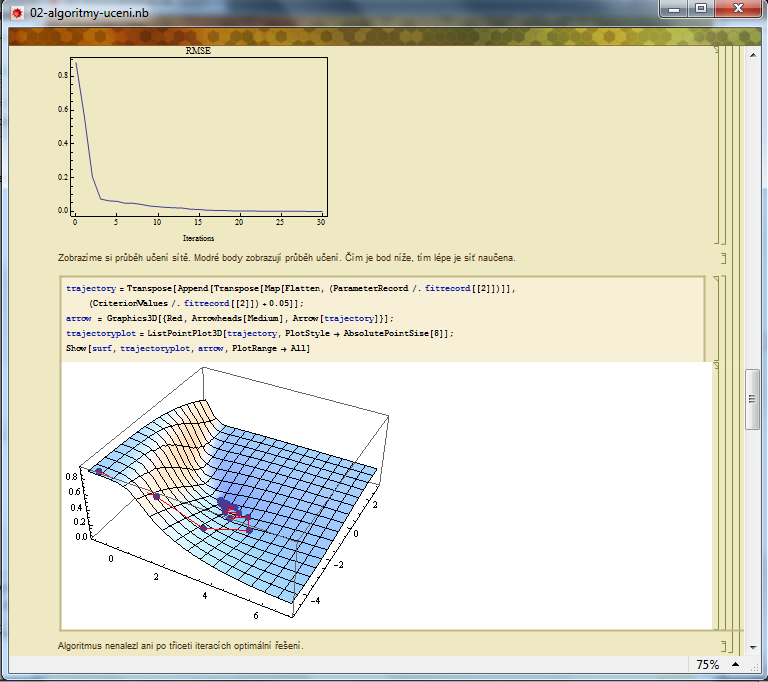
\includegraphics[height=10cm]{figures/ukazka02.png}
\caption{Ukázka souboru 02-algoritmy-uceni.nb}
\label{fig:algoritmy-uceni}
\end{center}
\end{figure}
\newpage
\section{Křížová validace}
V kapitole křížová validace seznamuji studenty s principem fungování křížové validace. Křížovou validaci ukazuji na Iris datech a jednoduché dopředné síti.

Nejprve jsem načetl data. Iris data jsem rozdělil na vstupní a výstupní vektory, výstupní vektory jsem zakódoval kódem 1 z N. Poté detailně rozebral předzpracování dat pro křížovou validaci. Dále jsem vytvořil neuronovou síť, kterou jsem pomocí křížové validace testoval. Následně jsem naimplementoval samotnou křížovou validaci. V této implementaci jsem vypisoval pro každý fold úspěšnost RMSE, kterou síť dosáhla. Po skončení všech kol křížové validace jsem zobrazil boxový graf s výsledky křížové validace viditelný na obrázku~\ref{fig:krossvalidace}. Po najetí myší na graf se k němu zobrazí legenda. Studentům jsem dal také možnost nechat si vypsat výsledky křížové validace v textovém formátu. Textový formát vypíše nejlepší výsledek, nejhorší výsledek a aritmetický průměr všech výsledků. Na závěr jsem dal studentům možnost provést si křížovou validaci vlastní sítě s vlastními daty. Vlastní křížové validaci nastaví student parametry jednoduchým přiřazením do proměnných, je potřeba aby  zadaná síť odpovídala zadaným vstupním a výstupním datům a data byla předzpracována pomocí postupu uvedeného v této kapitole. Tato kapitola se nachází v souboru \textit{03-krossvalidace.nb}.

\begin{figure}[h!]
\begin{center}
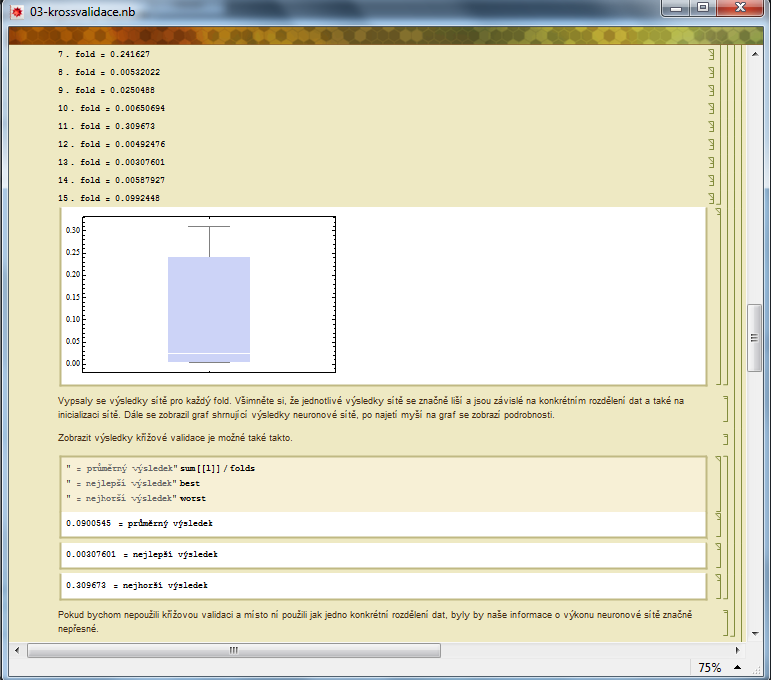
\includegraphics[height=10cm]{figures/ukazka03.png}
\caption{Ukázka souboru 03-krossvalidace.nb}
\label{fig:krossvalidace}
\end{center}
\end{figure}

\section{Dopředná síť}
\subsection{Jednoduchá data sin(x)}
V této kapitole poprvé seznamuji studenty s dopřednou neuronovou sítí. Funkci dopředné neuronové sítě jsem demonstroval na aproximaci funkce sinus.

Nejprve jsem připravil jednoduchá trénovací data navzorkováním funkce sinus na intervalu <0, 2\begin{math}\pi \end{math}>. Navzorkovaná data jsem pro jasnou představu zobrazil v textové i grafické podobě. Poté jsem ukázal jakým způsobem vytvořit neuronovou síť požadované struktury, jak si zobrazit dodatečné informace o síti a jak síť naučit na trénovacích datech. Dále jsem graficky zobrazil výstup sítě před naučením a po naučení jak je vidět na obrázku~\ref{fig:feedforward-sin}. Na závěr jsem ukázal jak převést síť do formy vzorce. Tato kapitola se nachází v souboru \textit{04-feedforward-sin.nb}.

\begin{figure}[h!]
\begin{center}
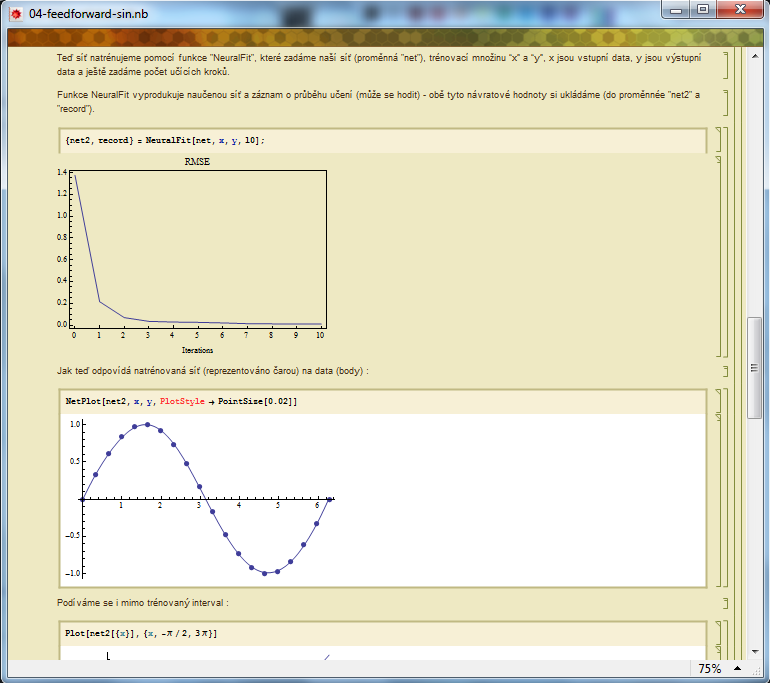
\includegraphics[height=10cm]{figures/ukazka04.png}
\caption{Ukázka souboru 04-feedforard-sin.nb}
\label{fig:feedforward-sin}
\end{center}
\end{figure}

Soubor vznikl úpravou souboru Petra Chlumského. Změnil jsem vzhled notebooku a upravil doprovodný komentář.

\subsection{Iris data}
V této kapitole ukazuji jakým způsobem pomocí dopředné sítě klasifikovat Iris data.

Nejprve jsem načetl data. Studentům jsme dal na výběr zda chtějí načíst data z internetu nebo použít lokální soubor s daty. Poté jsem data předzpracoval. Data jsem rozdělil na vstupní a výstupní vektory, protože výstupní parametr je textový, provedl jsem jeho překódování metodou 1 z N, kdy je každé třídě přiřazen jeden výstupní vektor. Toto předzpracování jsem prováděl krok po kroku s velmi podrobným komentářem a ještě jsem ho doplnil několika dalšími ukázkovými příklady. Po předzpracování dat jsem vytvořil dopřednou neuronovou síť, a data jsem touto neuronovou sítí zpracoval. Dále jsem zobrazil jak se vyvíjela úspěšnost klasifikace v průběhu učení (zobrazeno na obrázku~\ref{fig:feedforward-iris}). Na závěr jsem použil 3D graf, který ukazuje úspěšnost sítě na trénovacích datech (také ukázáno na obrázku~\ref{fig:feedforward-iris}). Také jsem ukázal možnost jak síť nechat symbolicky vyhodnotit. Tato kapitola se nachází v souboru \textit{05-feedforward-iris.nb}.

\begin{figure}[h!]
\begin{center}
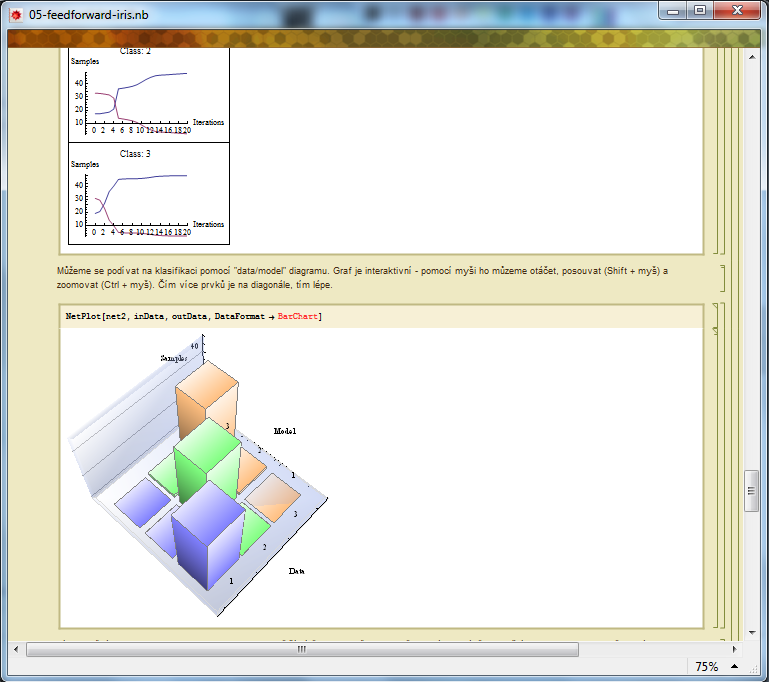
\includegraphics[height=10cm]{figures/ukazka05.png}
\caption{Ukázka souboru 05-feedforard-iris.nb}
\label{fig:feedforward-iris}
\end{center}
\end{figure}

Soubor vznikl úpravou souboru Petra Chlumského. Změnil jsem vzhled notebooku. V doprovodném komentáři jsem nahradil sousloví \uv{skupina v datech} slovem \uv{třída}, které podle mého názoru lépe vystihuje popisovanou skutečnost. Dále jsem komentář rozšířil. V závěru notebooku jsem nezobrazoval vývoj úspěšnosti klasifikace během učení ve 3D grafu, který podle mě nebyl tak přehledný a jasný jako 2D graf, který je zobrazen.

\subsection{Různé přístupy k učení sítě}
V tomto notebooku ukazuji několik různých přístupů k učení dopředné sítě. Tyto přístupy se liší hlavně v dělení dat na trénovací, testovací a validační množinu. Ukazuji také použití křížové validace a rozebírám vyhodnocení úspěšnosti neuronové sítě.

Nejprve jsem načetl Iris data a provedl jejich předzpracování stejně jako v minulé kapitole. Takto předzpracovaná data jsem náhodně rozdělil na trénovací, validační a testovací množinu. Ukázal jsem možnost použití křížové validace k určení vhodné struktury sítě. Při křížové validaci jsem výsledky sítí porovnával podle hodnoty RMSE, výsledky křížové validace jsem zobrazil v boxovém grafu, který je na obrázku~\ref{fig:feedforward-iris-2}. Síť, která vyšla z křížové validace nejlépe, jsem poté naučil na trénovací množině s použitím validační množiny. Validační množinu jsem použil k zastavení učení sítě, pokud by se úspěšnost klasifikace na validační množině začala v průběhu učení zhoršovat. Poté jsem vyhodnotil úspěšnost klasifikace na testovací množině. Tuto úspěšnost jsem pro snadnou čitelnost uvedl v procentech. Dále jsem síť se stejnou strukturou naučil bez použití validační množiny a taktéž jsem vyhodnotil její úspěšnost. Kapitola se nachází v souboru \textit{06-feedforward-iris-2}.

\begin{figure}[h!]
\begin{center}
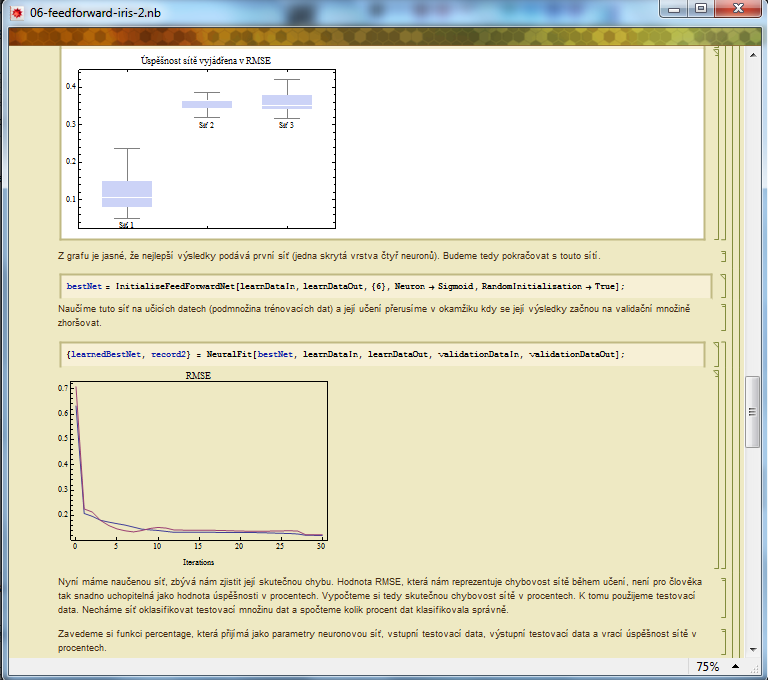
\includegraphics[height=10cm]{figures/ukazka06.png}
\caption{Ukázka souboru 06-feedforard-iris-2.nb}
\label{fig:feedforward-iris-2}
\end{center}
\end{figure}

\section{RBF síť}
\subsection{Ukázka výstupu skrytého neuronu}
Tato kapitola není určena přímo pro experimentování se sítí, ale spíše pro pochopení jakým způsobem RBF síť funguje. V notebooku zobrazuji výstup skrytého RBF neuronu.

Nejprve jsem vygeneroval vstupní data. Data jsou tvořena dvěma dobře oddělenými shluky, každý shluk představuje jednu třídu. Poté jsem vytvořil jednoduchou RBF neuronovou síť s jedním skrytým RBF neuronem, pomocí které jsem vstupní data klasifikoval. Síť jsem naučil na vygenerovaných datech, poté jsem zobrazil výstup RBF neuronu. Pro lepší představu o tom, jakým způsobem RBF neuron pokryl vstupní data, jsem tato data zobrazil společně s výstupem neuronu do jednoho grafu, který je na obrázku~\ref{fig:rbf-neuron}. Kapitola se nachází v souboru \textit{07-rbf-neuron.nb}.

\begin{figure}[h!]
\begin{center}
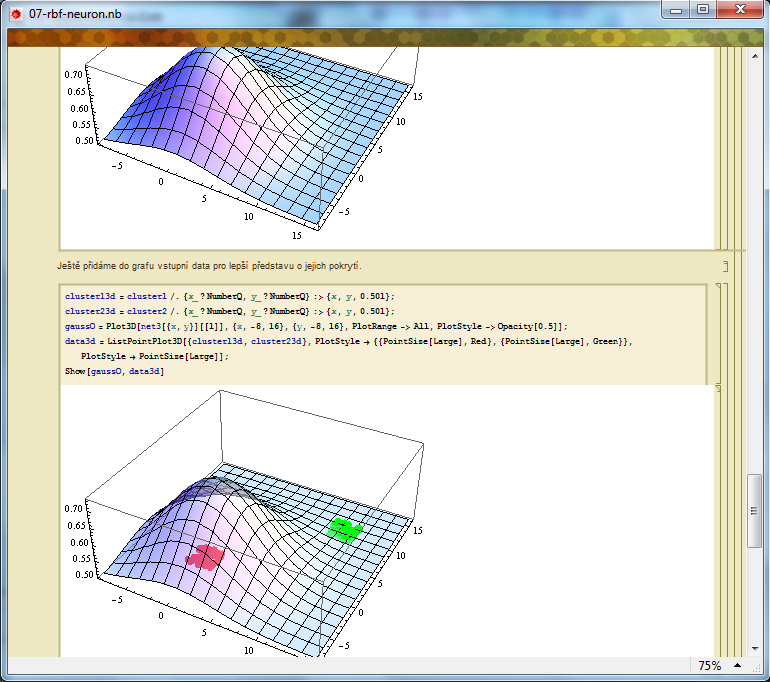
\includegraphics[height=10cm]{figures/ukazka07.png}
\caption{Ukázka souboru 07-rbf-neuron.nb}
\label{fig:rbf-neuron}
\end{center}
\end{figure}

\subsection{Ukázka výstupu tří skrytých neuronů}
Tato kapitola, stejně jako předchozí, slouží primárně k pochopení fungování RBF sítě. V notebooku zobrazuji výstup skryté vrstvy neuronů u RBF sítě se třemi RBF neurony, která je naučena na složitějších datech. 

Nejprve jsem vygeneroval data. Data se skládají ze šesti oddělených shluků, obsahují dvě třídy, každá třída se skládá ze třech shluků. Data jsem pro představu zobrazil v grafu. Dále jsem vytvořil RBF neuronovou síť, kterou jsem chtěl vygenerovaná data klasifikovat. Síť jsem naučil na vygenerovaných datech. Poté jsem zobrazil výstup neuronové sítě ve 2D i 3D grafu (zobrazeno na obrázku~\ref{fig:rbf-neuron2}), na kterých ukazuji jak síť klasifikuje data. Poté jsem zobrazen výstup skryté vrstvy RBF neuronů. Do stejného grafu s výstupem jednotlivých RBF neuronů jsem zobrazil i vstupní data, aby bylo vidět jak se RBF neurony přizpůsobily datům. Kapitola je v souboru \textit{08-rbf-neuron-2.nb}.

\begin{figure}[h!]
\begin{center}
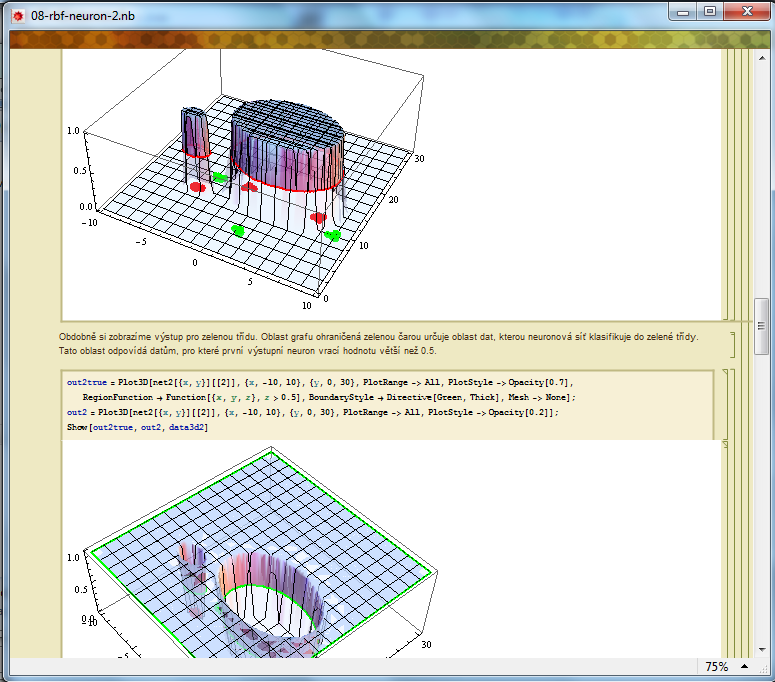
\includegraphics[height=10cm]{figures/ukazka08.png}
\caption{Ukázka souboru 08-rbf-neuron-2.nb}
\label{fig:rbf-neuron2}
\end{center}
\end{figure}

\subsection{Jednoduchá data sin(x)}
V této kapitole poprvé seznamuji studenty s RBF sítí. Ukazuji jak pomocí RBF sítě zpracovat jednoduchá data, v tomto případě se jedná o aproximaci funkce sinus.

Nejprve jsem vygeneroval data navzorkováním funkce sinus na intervalu <0, 2\begin{math}\pi \end{math}>. Data jsem zobrazil v grafické i textové podobě, aby o nich měli studenti dobrou představu. Dále jsem ukázal jak vytvořit RBF neuronovou síť požadované struktury, jak si o ní zobrazit podrobnější informace a jakým způsobem jí naučit na trénovacích datech. Dále ukazuji jak reagovala nenaučená síť (je vidět na obrázku~\ref{fig:rbf-sin}) na data a také jak reaguje naučená síť na stejná data. Na závěr jsem ukázal jak je možné nechat síť symbolicky vyhodnotit (zobrazit ji ve formě vzorce). Kapitola je v souboru \textit{09-rbf-sin.nb}.

\begin{figure}[h!]
\begin{center}
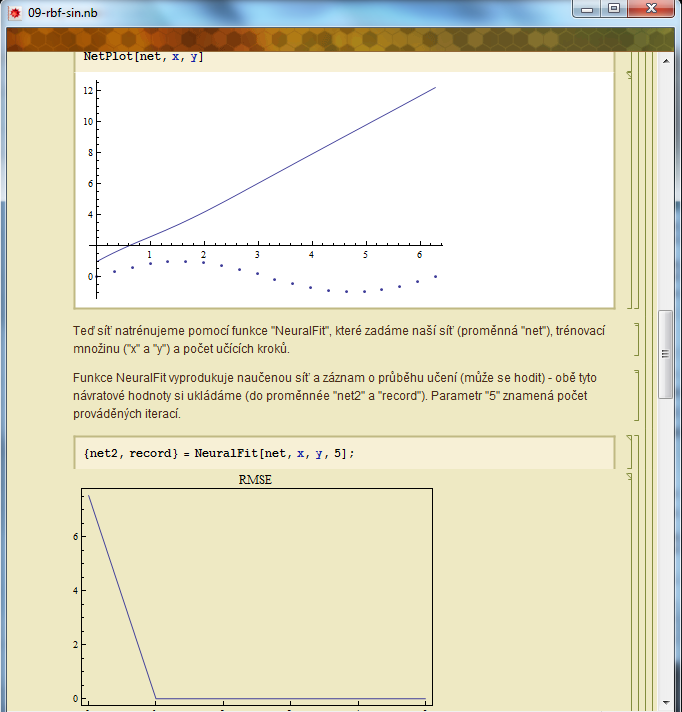
\includegraphics[height=10cm]{figures/ukazka09.png}
\caption{Ukázka souboru 09-rbf-sin.nb}
\label{fig:rbf-sin}
\end{center}
\end{figure}

Soubor vznikl úpravou souboru Petra Chlumského. Změnil jsem vzhled a rozšířil doprovodný komentář. Dále jsem odstranil nepřesné a nepravdivé popisky u vytváření RBF sítě a nahradil je správnou verzí.
\newpage
\subsection{Iris data}
Touto kapitolou ukazuji zpracování složitějších dat neuronovou sítí RBF. V notebooku provádím klasifikování Iris dat z UCI databáze \cite{UCI}.

Nejprve jsem načetl Iris data (opět jsem dal na výběr za je načíst ze souboru nebo z internetu), poté jsem provedl rozdělení dat na vstupní a výstupní vektory a výstupní data jsem zakódoval algoritmem 1 z N. Dále jsem vytvořil RBF síť, která jsem následně naučil na datech. Potom jsem zobrazil graf, který ukazuje jak se vyvíjela úspěšnost klasifikace v průběhu učení. Níže jsem ještě vykreslil graf porovnávající zadaná data s výstupem naší naučené RBF sítě. Na závěr jsem ukázal možnost symbolického vyhodnocení sítě. Kapitolu naleznete v souboru \textit{10-rbf-iris.nb}.

Soubor vznikl úpravou souboru Petra Chlumského. Změnil jsem grafický vzhled notebooku. Dále jsem významně zkrátil sekci předzpracování dat. V původním notebooku bylo předzpracování stejně rozsáhlé jako v souboru \textit{05-feedforward-iris.nb}, já ponechal pouze kód, který skutečně zpracovává Iris data a uvedl odkaz na soubor ve kterém je předzpracování popsáno podrobněji. Dále jsem na závěr notebooku nezobrazoval 3D graf s vývojem úspěšnosti klasifikace, který podle mého názoru není tolik vypovídající. Ponechal jsem 2D graf s vývojem klasifikace. Také jsem rozšířil komentář a opravil špatný popis u vytváření RBF sítě.
\subsection{Různé přístupy k učení sítě}
Kapitolou chci demonstrovat různé možnosti jak přistoupit k učení RBF sítě z hlediska rozdělení dat na trénovací, testovací a validační množinu. Také ukazuji možnost využití křížové validace k určení nejvhodnější struktury sítě. Na závěr ukazuji jak vyhodnotit úspěšnost sítě.

Nejprve jsem načetl Iris data (v notebooku jsem dal na výběr zda  ze souboru nebo z internetu). Načtená data jsem rozdělil na vstupní a výstupní vektory, výstupní vektory jsem překódoval kódem 1 z N. Takto zpracovaná data jsem rozdělil na trénovací, testovací a validační množinu. Dále jsem demonstroval možnost použití křížové validace, k určení nejvhodnější struktury sítě (v tomto případě k určení počtu RBF neuronů). Výsledek křížové validace jsem zobrazil v boxovém grafu. Dále jsem ukázal možnost učení RBF sítě s validační množinou. Validační množina slouží ke kontrole úspěšnosti sítě, jakmile se výsledky na validační množině zhorší oproti předchozí iteraci, je učení sítě ukončeno. Na testovacích datech jsem poté provedl určení skutečné úspěšnosti naučené sítě, kterou jsem vyjádřil v procentech. Dále jsem ukázal učení sítě bez použití validační množiny. U takto naučené sítě jsem také určil skutečnou úspěšnost na testovacích datech v procentech. Kapitola se nachází v souboru \textit{11-rbf-iris-2.nb}.
\section{Hopfieldova síť}
V této kapitole představuji studentům Hopfieldovou neuronovou síť a ukazuji její použití na jednoduchých datech.

Jako vstupní data jsem použil obrázky číslic 1, 2 a 3 zobrazené v poli 8x8, kde černá znamená 1 a bílá -1. Zobrazení dat můžete vidět na obrázku~\ref{fig:hopfield}. Tato data jsem zadal přímo v kódu. Poté jsem vytvořil Hopfieldovu síť, která jsem následně na vstupních datech naučil. Pro otestování, jak síť reaguje na data jsem potřeboval vytvořit testovací data, ta jsem vytvořil aplikací šumu na vstupní data. Tato zašuměná data jsem předložil naučené síti a zobrazil její reakci na ně. Na závěr jsem zobrazil graf ukazující jakým způsobem se minimalizovala energetická funkce pro jednotlivé předložené vzory. Kapitola se nalézá v souboru \textit{12-hopfield.nb}.

\begin{figure}[h!]
\begin{center}
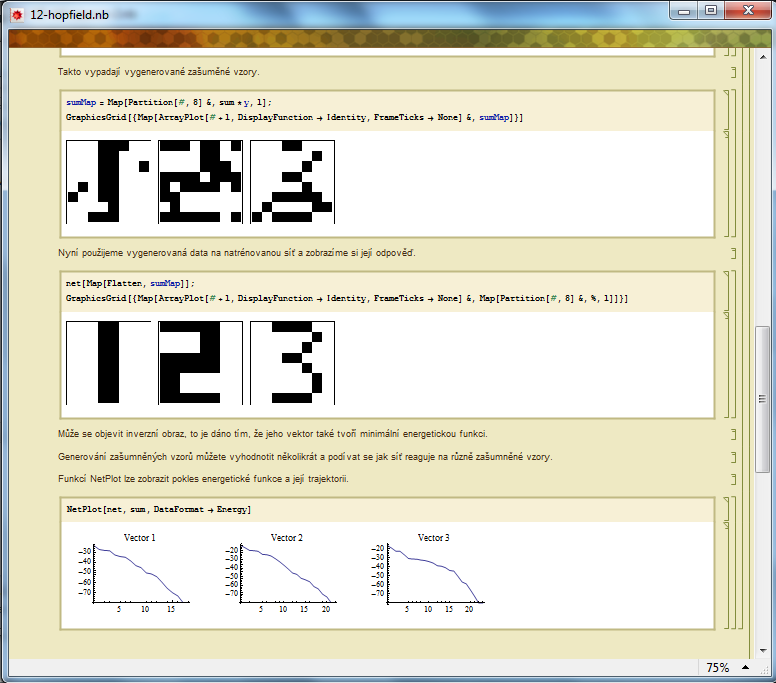
\includegraphics[height=10cm]{figures/ukazka12.png}
\caption{Ukázka souboru 12-hopfield.nb}
\label{fig:hopfield}
\end{center}
\end{figure}

Soubor vznikl úpravou souboru Petra Chlumského. Mimo úpravy celkového vzhledu notebooku a drobných úprav doprovodného komentáře spočívá hlavní úprava v nahrazení funkce GraphicsArray funkcí GraphicsGrid. Funkce GraphicsArray je v Mathematice 8 zastaralá a nedoporučuje se používat. Také jsem upravil funkci pro aplikaci šumu, která nyní zašumí předložený vzor o trochu více než tomu bylo dříve.
\newpage
\section{Samoorganizující mapy}
\subsection{Shlukování dat}
V této kapitole seznamuji studenty se samoorganizující se mapou a ukazuji její použití na jednoduchých datech. Pomocí samoorganizující se mapy hledám shluky ve vygenerovaných datech.

Na začátku jsem vygeneroval vstupní data. Data obsahují šest dobře oddělených shluků. V těchto datech jsem hledal pomocí samoorganizující se mapy šest shluků. Nejprve jsem vytvořil náhodně inicializovanou samoorganizující se mapu, kterou jsem naučil na vstupních datech. Pomocí grafu jsem zobrazil její výstup (tedy jak síť rozdělila data na shluky). Dále jsem ukázal jak odstranit ze sítě nepotřebný (mrtvý) neuron a zobrazil jsem výstup sítě bez nepotřebného neuronu. Následně jsem ukázal postup umožňující dosažení lepších výsledků. Samoorganizující se mapa jsem neinicializoval náhodně, ale použil jsem k její inicializaci metodou SOM. Poté jsem síť doučil na vstupních datech a graficky zobrazil její výstup, který je zobrazen na obrázku~\ref{fig:som-clustering}. Na závěr jsem zobrazil průběh učení obou sítí. Nejprve ve formě statického grafu, který zobrazuje trajektorii jednotlivých neuronů v průběhu učení. Podruhé jako interaktivní graf zobrazující výstup sítě pro danou iteraci. Pomocí posuvníku je možné vybírat, která iterace je zobrazena. Kapitola se nachází v souboru \textit{13-som-clustering.nb}.

\begin{figure}[h!]
\begin{center}
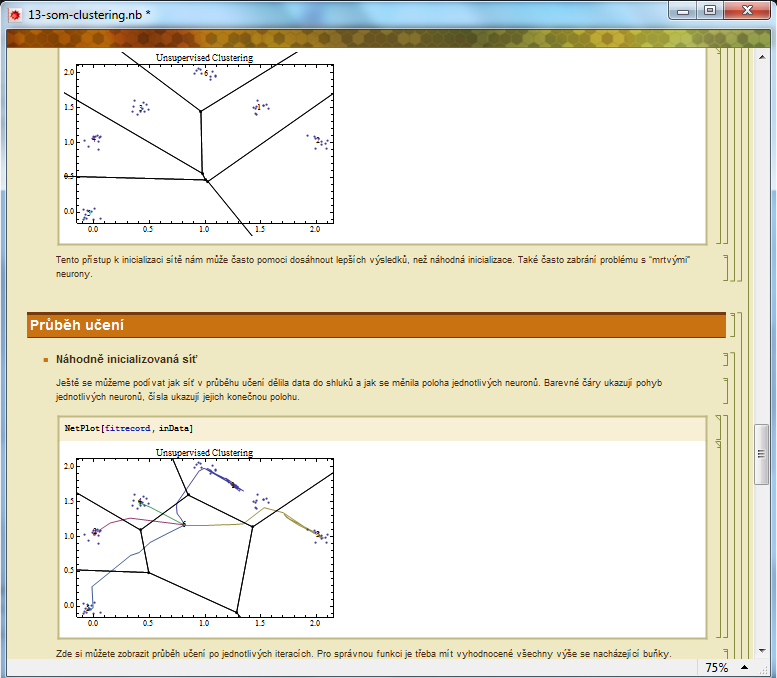
\includegraphics[height=10cm]{figures/ukazka13.png}
\caption{Ukázka souboru 13-som-clustering.nb}
\label{fig:som-clustering}
\end{center}
\end{figure}

\subsection{SOM a Iris data}
Touto kapitolou demonstruji použití samoorganizující se mapy na složitějších datech. K ukázce použití jsem z zvolil Iris data.

Nejprve jsem načetl Iris data(studentům jsem dal možnost načtení ze souboru nebo z internetu). Data jsem rozdělil na vstupní a výstupní vektory, výstupní vektory jsem překódoval metodou 1 z N. Dále jsem vytvořil samoorganizující se mapu, kterou jsem naučil na vstupních datech. Tento graf můžete vidět na obrázku~\ref{fig:som-iris}. Poté jsem vykreslil graf, který zobrazuje kolik vektorů náleží ke každému neuronu v síti. Stejným způsobem jsem zobrazil i průběh učení sítě. Následně jsem ukázal jakým způsobem lze libovolnému vektoru přiřadit jeho reprezentanta, jak spočítat Eukleidovskou vzdálenost od reprezentanta a také jsem připomněl mazání nepotřebných neuronů. Na závěr jsem rozebral doučování sítě. Kapitola se nalézá v souboru \textit{14-som-iris.nb}.

\begin{figure}[h!]
\begin{center}
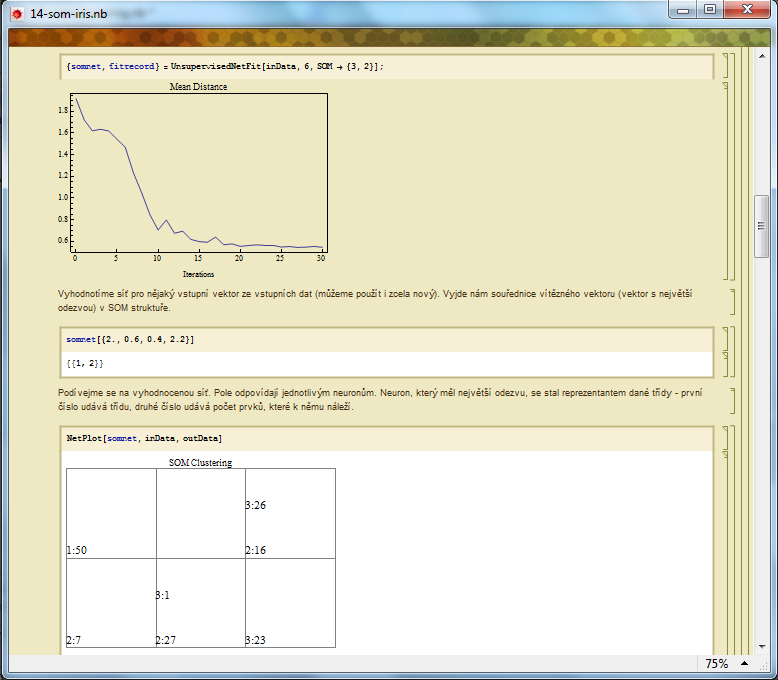
\includegraphics[height=10cm]{figures/ukazka14.png}
\caption{Ukázka souboru 14-som-iris.nb}
\label{fig:som-iris}
\end{center}
\end{figure}

Soubor vznikl úpravou souboru Petra Chlumského. Změnil jsem celkový vzhled notebooku, v komentáři jsem nahradil slovo \uv{skupina} slovem \uv{třída}, které podle mě lépe vystihuje popisovanou věc. Udělal jsem ještě několik menších úprav a rozšíření v komentáři. Dále jsem provedl úpravu předzpracování dat, které bylo zbytečně rozsáhlé a tím pádem zdlouhavé. Ponechal jsem pouze minimální potřebný kód a uvedl odkaz na notebook ve kterém je předzpracování dat detailně popsáno.
\section{LVQ}
V poslední kapitole seznamuji studenty s použitím LVQ sítě. Použití LVQ sítě je ukázáno na klasifikaci Iris dat.

Nejprve jsem načetl Iris data (dávám možnost načtení ze souboru nebo z internetu), data jsem rozdělil na vstupní a výstupní vektory a výstupní vektory jsem překódoval metodou 1 z N. Nejprve jsem nabídl několik pohledů na vstupní data (jeden z nich je na obrázku~\ref{fig:lvq}, společně s vytvořením LVQ sítě), poté jsem vytvořil LVQ síť, kterou jsem naučil na vstupních datech. Poté jsem zobrazil vizualizaci výstupu sítě v průběhu učení. Následně jsem ukázal jakým způsobem smazat nepotřebné neurony. Dále jsem demonstroval jak je možné nechat oklasifikovat libovolný vektor. Poté jsem zobrazil procentuální úspěšnost klasifikace. Na závěr jsem rozebral možnosti doučování sítě a ukázal několik možných grafických výstupů sítě. Tato kapitola se nachází v souboru \textit{15-lvq-iris.nb}.

\begin{figure}[h!]
\begin{center}
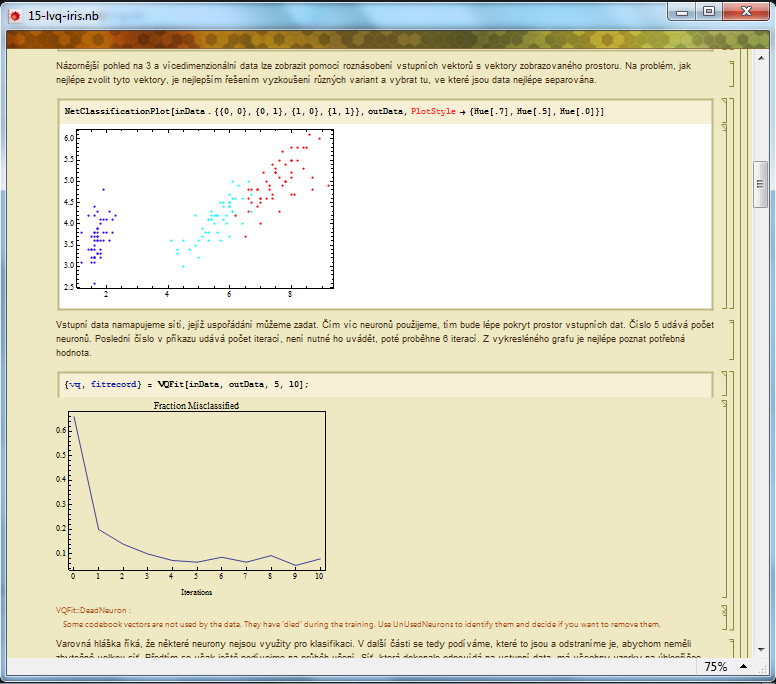
\includegraphics[height=10cm]{figures/ukazka15.png}
\caption{Ukázka souboru 15-lvq.nb}
\label{fig:lvq}
\end{center}
\end{figure}

Soubor vznikl úpravou souboru Petra Chlumského. Změnil jsem grafickou podobu notebooku. V doprovodném komentáři jsem nahradil slovo \uv{skupina} slovem \uv{třída}, které lépe vystihuje popisovanou skutečnost. Komentář jsem ještě drobně rozšířil a upravil. Upravil jsem a výrazně zkrátil předzpracování dat. Ponechal jsem pouze kód, který skutečně manipuluje s daty a uvedl odkaz na notebook, ve kterém se nachází detailně popsaný proces předzpracování dat. 
%*****************************************************************************
\chapter{Závěr}
V rámci své bakalářské práce jsem rozšířil demonstrační aplikaci pro podporu výuky neuronových sítí na FEL ČVUT. Původní aplikace se skládala z 8 souborů, já jsem ji rozšířil na 15 souborů a soubory původní aplikace jsem upravil a částečné přepracoval. Původní aplikace pokrývala základní práci s dopřednou, RBF, Hopfieldovou, Kohonenovou a LVQ sítí. Já jsem ji rozšířil o demonstraci různých trénovacích algoritmů, křížovou validaci, ukázal jsem různé přístupy k učení sítě z pohledu dělení dat na validační, trénovací a testovaní množinu a podrobně jsem rozebral \uv{vnitřnosti} RBF neuronové sítě. Součástí práce je také teoretická část, ve které jsem popsal základní principy a strukturu vybraných neuronových sítí.

Díky bakalářské jsem si značně rozšířil své znalosti neuronových sítí a také jsem rozšířil své schopnosti programovat v systému Mathematica, se kterým jsem měl do té doby pouze pasivní zkušenosti.

Cíle bakalářské práce se mi podařilo naplnit. Výstup této práce bude použit ve cvičeních předmětu \uv{Neuronové sítě a neuropočítače}.
%*****************************************************************************
% Seznam literatury je v samostatnem souboru reference.bib. Ten
% upravte dle vlastnich potreb, potom zpracujte (a do textu
% zapracujte) pomoci prikazu bibtex a nasledne pdflatex (nebo
% latex). Druhy z nich alespon 2x, aby se poresily odkazy.

% originally following specification for bibliography formating was used
%\bibliographystyle{abbrv}

% Here is an improvment by Petr Dlouhy (April 2010).
% It is mainly for supervisors who expect Czech fomrating rules for references
% Additional feature is live url addresses to sources from your pdf file
% It requires the file csplainnat.bst (included in this sample zipfile).

\bibliographystyle{csplainnat}

%bibliographystyle{plain}
%\bibliographystyle{psc}
{
%JZ: 11.12.2008 Kdo chce mit v techto ukazkovych odkazech take odkaz na CSTeX:
\def\CS{$\cal C\kern-0.1667em\lower.5ex\hbox{$\cal S$}\kern-0.075em $}
\bibliography{reference}
}

% M. Dušek radi:
%\bibliographystyle{alpha}
% kdy citace ma tvar [AutorRok] (napriklad [Cook97]). Sice to asi neni  podle ceske normy (BTW BibTeX stejne neodpovida ceske norme), ale je to nejprehlednejsi.
% 3.5.2009 JZ polemizuje: BibTeX neobvinujte, napiste a poskytnete nam styl (.bst) splnujici citacni normu CSN/ISO.

%*****************************************************************************
%*****************************************************************************
\appendix


%*****************************************************************************
%\chapter{Seznam použitých zkratek}

%\begin{description}
%\item[2D] Two-Dimensional
%\item[ABN] Abstract Boolean Networks
%\item[ASIC] Application-Specific Integrated Circuit
%\end{description}
%\vdots


%*****************************************************************************
\chapter{Obsah přiloženého CD}
\textbf{\large Tato příloha je povinná pro každou práci. Každá práce musí totiž obsahovat přiložené CD. Viz dále.}

Může vypadat například takto. Váš seznam samozřejmě bude odpovídat typu vaší práce. (viz \cite{infodp}):

\begin{figure}[h]
\begin{center}
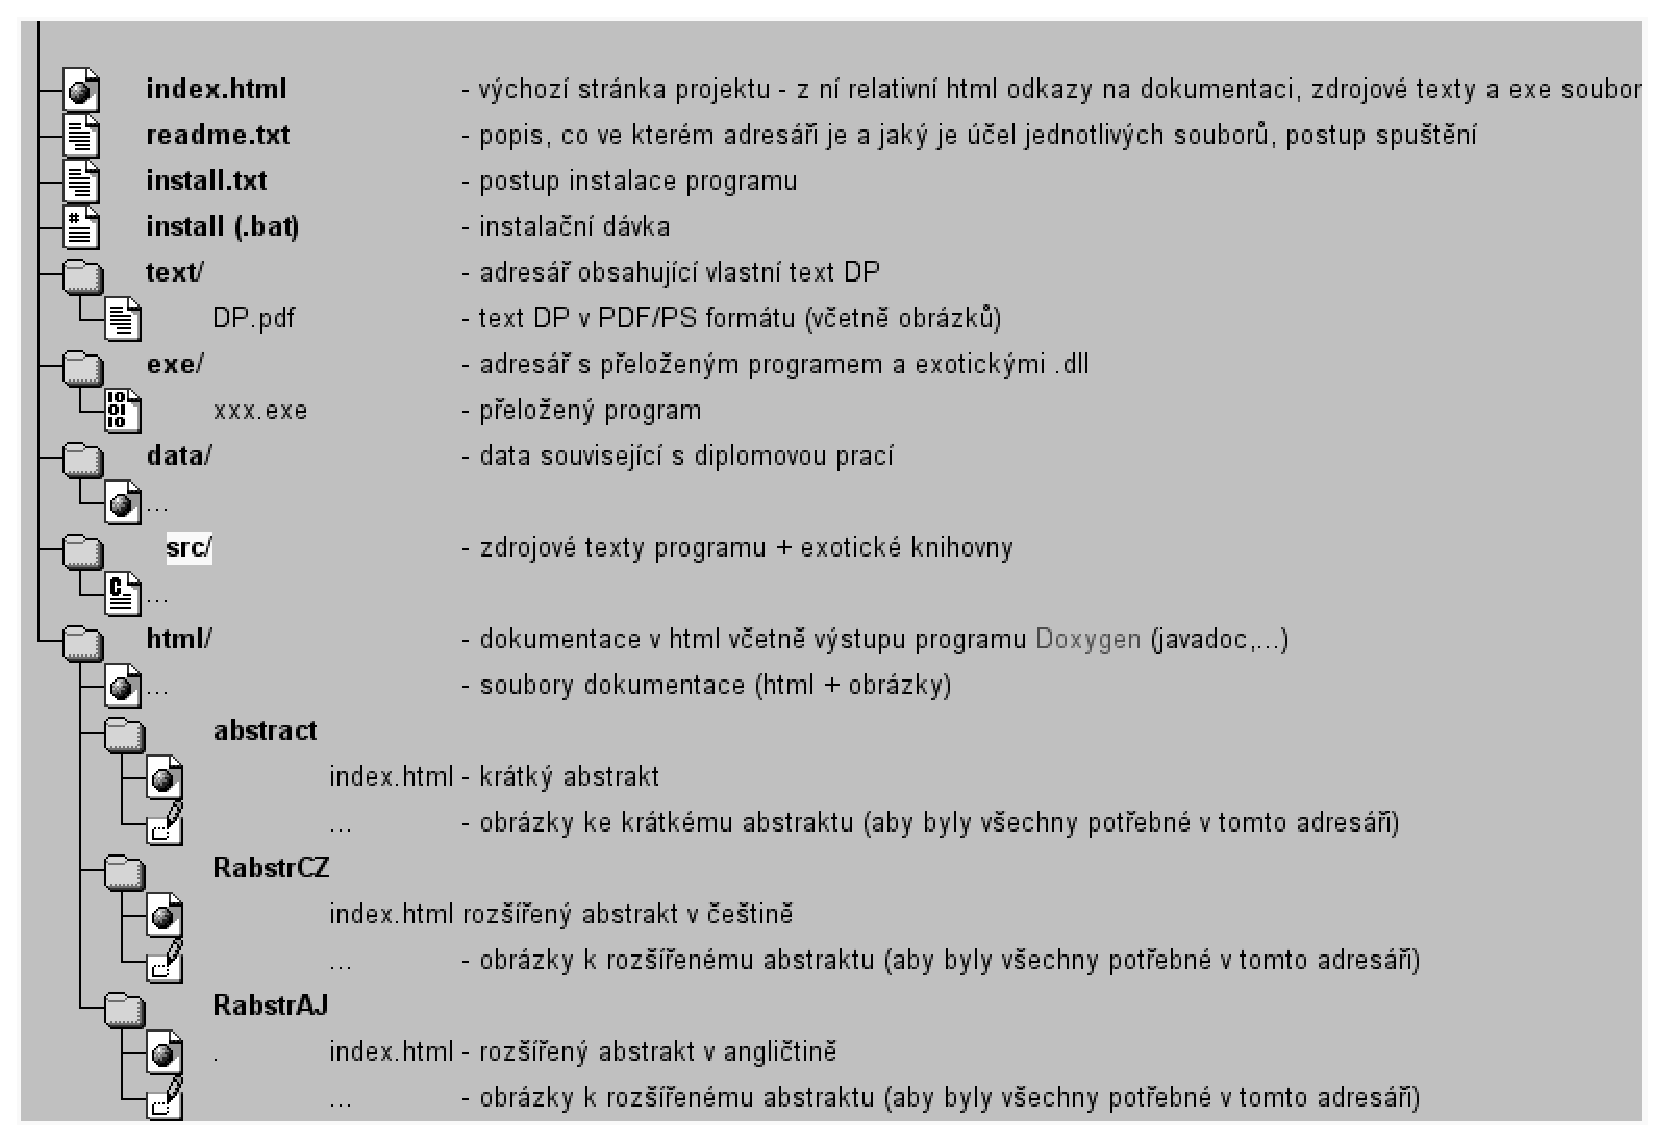
\includegraphics[width=14cm]{figures/seznamcd}
\caption{Seznam přiloženého CD --- příklad}
\label{fig:seznamcd}
\end{center}
\end{figure}

Na GNU/Linuxu si strukturu přiloženého CD můžete snadno vyrobit příkazem:\\ 
\verb|$ tree . >tree.txt|\\
Ve vzniklém souboru pak stačí pouze doplnit komentáře.

Z \textbf{README.TXT} (případne index.html apod.)  musí být rovněž zřejmé, jak programy instalovat, spouštět a jaké požadavky mají tyto programy na hardware.

Adresář \textbf{text}  musí obsahovat soubor s vlastním textem práce v PDF nebo PS formátu, který bude později použit pro prezentaci diplomové práce na WWW.

\end{document}
